\documentclass[10pt,twocolumn,letterpaper]{article}

% \usepackage{cvpr}
\usepackage{times}
\usepackage{epsfig}
\usepackage{graphicx}
\usepackage{amsmath}
\usepackage{amssymb}
\usepackage{makecell}

% Include other packages here, before hyperref.
\usepackage{subfig}
\newcommand{\subsubfloat}[2]{%
  \begin{tabular}{@{}c@{}}#1\\#2\end{tabular}%
}

% If you comment hyperref and then uncomment it, you should delete
% egpaper.aux before re-running latex.  (Or just hit 'q' on the first latex
% run, let it finish, and you should be clear).
\usepackage[breaklinks=true,bookmarks=false]{hyperref}
\usepackage{multirow}
\DeclareMathOperator*{\argmin}{argmin}
\DeclareMathOperator*{\argmax}{argmax}


\begin{document}
%%%%%%%%% Preface
\onecolumn
\pagenumbering{gobble}
% \chapter{Preface}


Transferring pre-trained representations is widely adopted by convolutional neural networks for semantic segmentation because the training data is often available only on a small scale.
In domains where directly adapting classification networks is challenging, we propose to train representations with segmentation datasets containing mislabeled objects and unsegmented objects.
Our experiments demonstrate that both mislabeled segments and incomplete segmentation lower the fine-tuning performance of the learned representations.
To get rid of the negative effect of objects label noises, we propose to assign objects of any categories a foreground label instead of the exact object categories.
Learning representations by segmenting foreground and background turns out to improve the fine-tuning performance significantly when label noises are dominant in the pre-training data.
In the existence of unsegmented objects, a sigmoid loss for the background class is proposed to achieve high recall while keeping the precision better than simply weighting the classes.
The proposed class dependent, sigmoid loss achieves both better pre-training performance and better fine-tuning performance than the class-weighted loss in the presence of incomplete segmentation.


Members of the thesis committee include Prof. dr. A.Hanjalic (Multimedia Computing Group, TU Delft) as the chair, dr. J.C. van Gemert (Vision Lab, TU Delft) who was the daily supervisor of the student, and Prof.dr. M. Loog  (Pattern Recognition Laboratory, TU Delft) and dr. Z. Szlávik (CAS Benelux, IBM).

I sincerely appreciate the magnificent supports provided by dr. J.C. van Gemert, Prof.dr. M. Loog and dr. Z. Szlávik as co-supervisors day to day.
I would also like to thank dr. D.M.J. Tax for his expert knowledge in the domain.

\begin{flushright}
{\makeatletter\itshape
    Jihong Ju \\
    Delft, \today
\makeatother}
\end{flushright}


%%%%%%%%% TITLE
\twocolumn
\pagenumbering{arabic}
\newpage
\title{Learn transferable features with noisy segmentation datasets}

\author{First Author\\
Institution1\\
Institution1 address\\
{\tt\small firstauthor@i1.org}
% For a paper whose authors are all at the same institution,
% omit the following lines up until the closing ``}''.
% Additional authors and addresses can be added with ``\and'',
% just like the second author.
% To save space, use either the email address or home page, not both
\and
Second Author\\
Institution2\\
First line of institution2 address\\
{\tt\small secondauthor@i2.org}
}

\maketitle
%\thispagestyle{empty}


%%%%%%%%% ABSTRACT
\begin{abstract}

% Noisy data exists
% Transfer learning
% Noises affect feature transferability
% Binarizing classes
% Modify loss for incomplete segmentation

The broad existence of noisy datasets motivates us to consider if it is possible to utilize noisy segmentations in training better image segmentation models with limited training samples.
We investigated in this work to pre-train convolutional neural network (CNN) models with potential incomplete, mislabeled segmentations.
The influence of segmentation noises on model transferability was investigated in an experimental setup with synthesized segmentation noises.
With the same setup, we discovered that binarizing classes as foreground and background could improve feature transferability for a small training set corrupted heavily with random labels.
A class-dependent modification to the cross-entropy loss was proposed to balance precision and recall for training with incomplete segmentations.
Compared to simply changing class weights, the proposed sigmoidal loss down-weights the losses for confident predictions and unconfident predictions differently.
Experiments demonstrated that replacing the cross-entropy loss with a sigmoidal loss for background class provide an improvement to both pre-training and fine-tuning performance in the presence of incomplete segmentation.\end{abstract}

%%%%%%%%% BODY TEXT

\section{Introduction}
\label{introduction}



%%%%%%%%%%%%%%%%%%%%%%%%%%%%%%%%%%%%%%%%%%%%%%%%%%%%%%%%%%%%%%%%%%%%%%
%%%%%%%% Figure 1
%%%%%%%%%%%%%%%%%%%%%%%%%%%%%%%%%%%%%%%%%%%%%%%%%%%%%%%%%%%%%%%%%%%%%%

\begin{figure}[t]
\begin{center}
% \fbox{\rule{0pt}{2in} \rule{0.9\linewidth}{0pt}}
   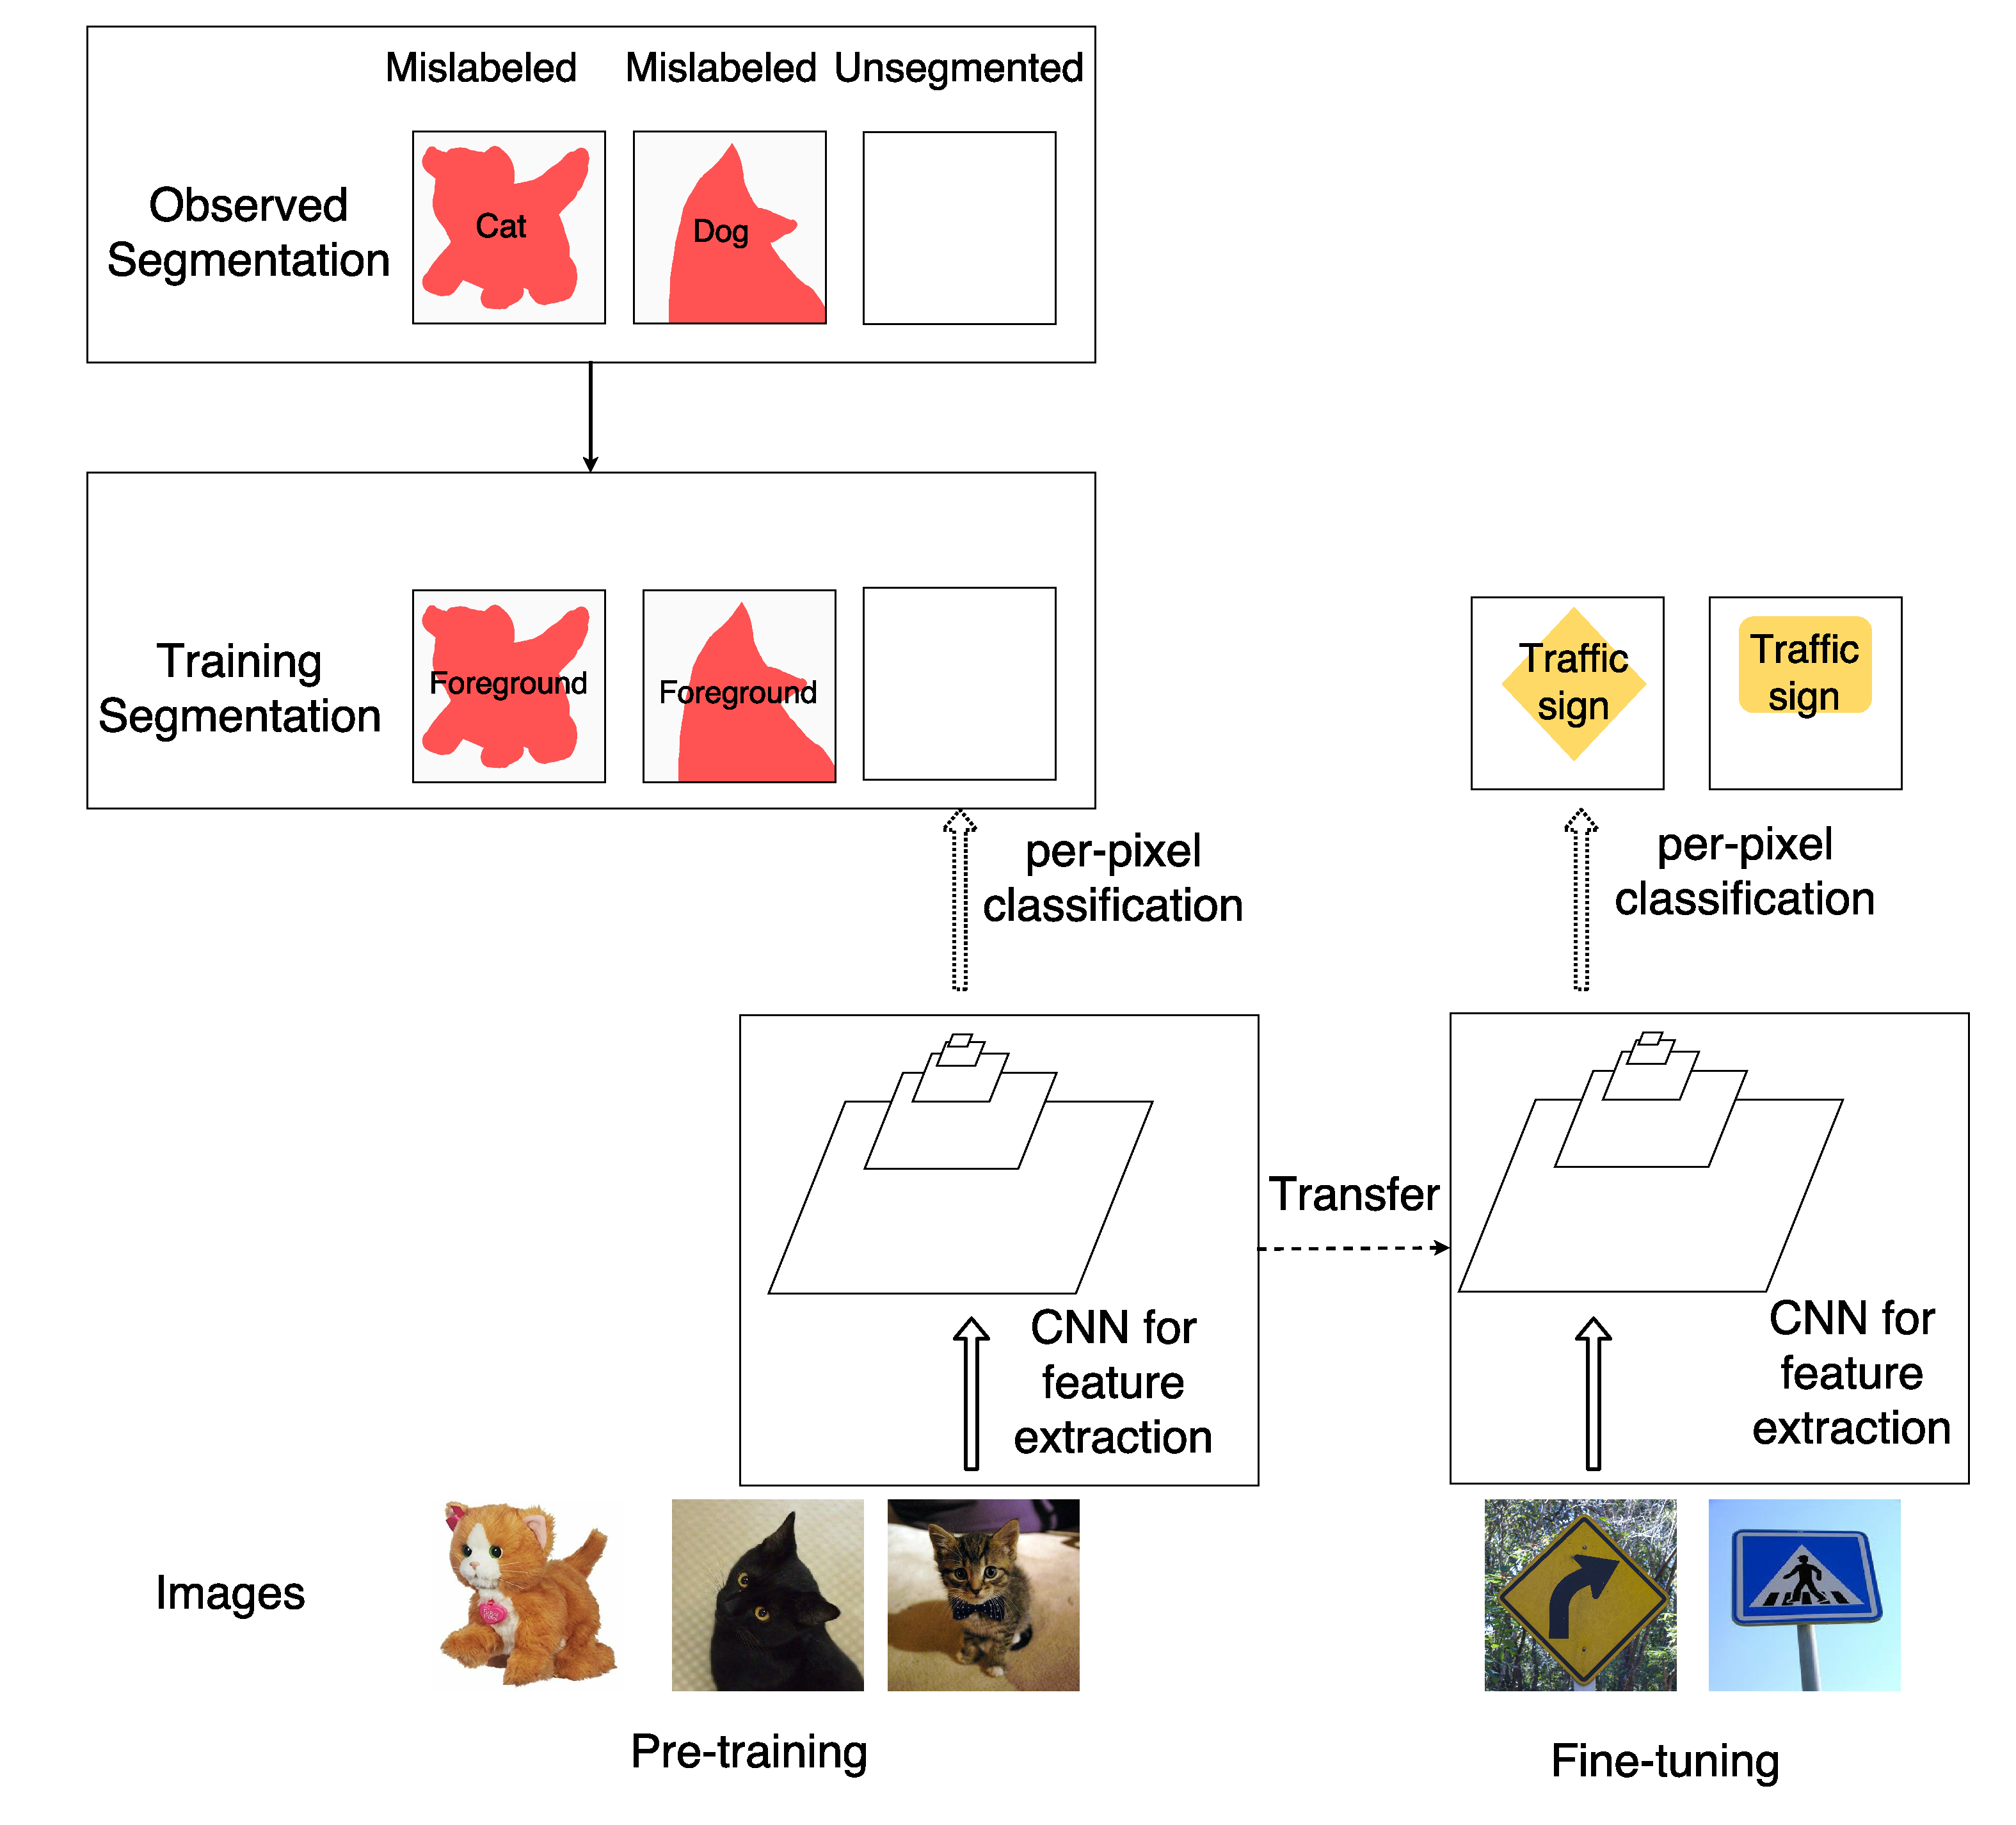
\includegraphics[width=1.0\linewidth]{img/figure1}
\end{center}
   \caption{
   Learning representations with segmentation datasets that potentially contains mislabeled objects and missing segmentation.
   We propose (1) to train with only segmentations instead of labeled segmentations, (2) to apply a sigmoid loss for the background class.
   The learned representations are then used as weights initialization and fine-tuned with a small set of true labels in the domain of interest.
   }
\label{fig:figure1}
\end{figure}


%%%%%%%%%%%%%%%%%%%%%%%%%%%%%%%%%%%%%%%%%%%%%%%%%%%%%%%%%%%%%%%%%%%%%%
%%%%%%%% TEXT Why transfer learning?
%%%%%%%%%%%%%%%%%%%%%%%%%%%%%%%%%%%%%%%%%%%%%%%%%%%%%%%%%%%%%%%%%%%%%%

% \noindent \textit{Why transfer learning? \\
% Segmentation model benefits from transfer learning.
% \begin{itemize}
%   \item Success of CNN benefits from large-scale data whereas segmentation datasets are small
%   \item Collecting segmentation in one domain on a large scale can be difficult.
%   \item One can transfer pre-trained CNN model to train with limited training samples access.
% \end{itemize}
% }

The often limited availability of training samples motivates most state-or-the-art deep learning based segmentation models \cite{long2015fully,chen2016deeplab,he2017mask} to transfer convolutional neural network (CNN) models \cite{krizhevsky2012imagenet,simonyan2014very,szegedy2015going,he2016deep} trained on a subset of images from ImageNet.
% The pre-trained models \cite{krizhevsky2012imagenet,simonyan2014very,szegedy2015going,he2016deep} are normally trained on an object recognition task, the ILSVRC \cite{russakovsky2015imagenet} challenge, using around 1.2 million labeled images.
% Compared to object recognition tasks, it is tougher to collect a dataset for semantic segmentation on a large scale.
The difficulty of obtaining manual segmentations is natural because it costs much more efforts for people to segment than to classify an image.
One of the largest segmentation datasets, Microsoft COCO2014 \cite{lin2014microsoft}, contains 123,287 images of 80 object categories.
As a comparison, a well-known successful task for convolutional neural networks, object recognition on the ILSRVC dataset\cite{russakovsky2015imagenet}, has around 1.2 million images for 1000 categories to train.
% the Pascal VOC2012 challenge \cite{everingham2015pascal} provides a segmentation dataset with only 9,993 segmented images for 20 object categories;
% The PASCAL-context Dataset \cite{mottaghi2014role} enriches the PASCAL VOC dataset by segmenting all 11,530 training images for 540 categories;
Transferring weights from the pre-trained ImageNet models can provide a segmentation performance boost in the limitation of lacking training samples, as reported in \cite{long2015fully} and adopted by \cite{chen2016deeplab,he2017mask}.
But the pre-trained ImageNet models are originally designed for object recognition problems, which can cause more problems than it solves.

%%%%%%%%%%%%%%%%%%%%%%%%%%%%%%%%%%%%%%%%%%%%%%%%%%%%%%%%%%%%%%%%%%%%%%
%%%%%%%% TEXT Why pre-training with segmentation?
%%%%%%%%%%%%%%%%%%%%%%%%%%%%%%%%%%%%%%%%%%%%%%%%%%%%%%%%%%%%%%%%%%%%%%

% \noindent \textit{Why pre-training with segmentation? \\
% ImageNet models have limitations.
% \begin{itemize}
%   \item Disimilarity in domain of interest for training images
%   \item Architecture limitation of ImageNet models. (3D ConvNet)
% \end{itemize}
% }

In practice, it can be challenging to employ representations from the ImageNet CNN models directly for segmentation.
Firstly, the object recognition models pursue features invariance to better capture semantics regardless the variations in objects.
The result translation invariant and resolution-reduced features reduce the localization accuracy which is not essential for object recognition but is critical for object segmentation. \cite{zheng2015conditional,chen2016deeplab}
Secondly, the ImageNet models were originally trained with natural images at relatively low resolution.
However, images to be segmented may (1) have a third dimension (3D images like CT scans and MRI scans), (2) contain extra channels (RGB-D images),  (3) be non-natural, such as aerial images and medical images.
These issues prevent transferring representations of the ImageNet models from improving segmentation performance significantly.
In this case, it can be beneficial to retrain the pre-trained ImageNet models with segmentation datasets for fine-grained cues about boundaries in the domain.

% \footnote{The KITTI Vision Benchmark Suite http://www.cvlibs.net/datasets/kitti/}

%%%%%%%% ? Deeplab https://arxiv.org/pdf/1606.00915.pdf
%%%%%%%% In particular we consider three challenges in the application of DCNNs to semantic image segmentation: (1) reduced feature resolution, (2) existence of objects at multiple scales, and (3) reduced localization accuracy due to DCNN invariance.
%%%%%%%% ? CRFasRNN http://www.robots.ox.ac.uk/~szheng/papers/CRFasRNN.pdf
%%%%%%%% Firstly, traditionalCNNs have convolutional filters with large receptivefields and hence produce coarse outputs when restructured to produce pixel-level labels [37]
%%%%%%%% Secondly, CNNs lack smoothness constraints that encourage label agreement between similar pixels, and spatial and appearance consistency of the labelling output


%%%%%%%%%%%%%%%%%%%%%%%%%%%%%%%%%%%%%%%%%%%%%%%%%%%%%%%%%%%%%%%%%%%%%%
%%%%%%%% TEXT Why labels are noisy?
%%%%%%%%%%%%%%%%%%%%%%%%%%%%%%%%%%%%%%%%%%%%%%%%%%%%%%%%%%%%%%%%%%%%%%

% \noindent
% \textit{Why labels are noisy?
% \begin{itemize}
%   \item Crowd-sourcing data is noisy by nature.
%   \item ``gold standard'' itself can be ambiguous.
%   \item There exists free available noisy segmentation datasets
% \end{itemize}
% }

The segmentation datasets for pre-training representations may contain label errors.
The use of the crowd-sourcing platform like Mechanical Turk is common nowadays to collect annotations on a large-scale.
It is natural for crowd-sourcing workers to make mistakes as a result of lack of expertise, inherent ambiguity of tasks or unconscious bias.
Enormous efforts are required, according to  \cite{lin2014microsoft,everingham2015pascal}, to ensure the correctness of segmentations.
%A slight decrease in the percentage of segmentation errors, such as from 1\% to 0\%, may require extraordinary extra efforts due to the difficulty of identifying errors.
% If not requiring ``gold standard'' segmentations for training, the efforts saved for correctness can be made to segment more images for a larger dataset.
%In some domains, for example, medical imaging, the ``gold standard'' itself can be ambiguous and cause disagreements among experts.
In addition, automated labels other than the manual ones may be freely available for particular tasks.
For example, segmentations of road and buildings for aerial images can be derived from digital maps, like OpenStreetMap, by aligning images to maps.
However, segmentations constructed in this way suffer from incompleteness as well as registration problems \cite{mnih2012learning}.
% Besides, Pl@ntNet\footnote{https://identify.plantnet-project.org/}, a crowdsourcing platform, provide millions of images of plants and corresponding labels which may or may not be correct.
Ideally, label errors in segmentations should not significantly affect the learned representations and its transferability to other datasets.

%%%%%%%%%%%%%%%%%%%%%%%%%%%%%%%%%%%%%%%%%%%%%%%%%%%%%%%%%%%%%%%%%%%%%%
%%%%%%%% TEXT What types of noises exist and motivate them?
%%%%%%%%%%%%%%%%%%%%%%%%%%%%%%%%%%%%%%%%%%%%%%%%%%%%%%%%%%%%%%%%%%%%%%

% \noindent \textit{What types of noises exist and motivate them?
% \begin{itemize}
%   \item Inexaustive segmentation
%   \item Misclassification
%   \item False segmentations
% \end{itemize}
% }

% \paragraph{Segmentation noises}

Label errors of different kinds can exist in segmentation labels.
We consider mislabelling errors occurred to the whole segment instead of individual pixels, assuming the outline of objects is always correct.
This is based on the observations that most objects in natural images have visually clear borders, and it may be untrue in some cases, for example, context segmentations\cite{mottaghi2014role}.
In particular, we consider three types of label errors: inexhaustive segmentation, objects mislabelling, and false positive segmentations.
\textbf{Objects mislabelling} from one category to another exist occasionally even for well-annotated datasets.
For example, the Microsoft COCO dataset \cite{lin2014microsoft} contains some mislabeled cats and dogs even though annotators were asked to segment only one category at a time;
\textbf{Inexhaustive segmentation} means that there exist objects left unsegmented.
A typical scenario where incomplete segmentation emerges is to segment images containing massive amounts of objects of the same kind, e.g., a flock of sheep or a pile of products;
\textbf{False positive segmentation} denotes that semantically meaningful objects from an undefined category are wrongly segmented, as objects of interest.
For instance, a dataset may contain segmentations for toy cats, labeled cats, given that toy is not one of the categories of interest and cat is.
We report in this work that objects mislabelling and inexhaustive segmentation both have a negative influence on the learned representations, whereas the false positive segmentation has little effects.


%%%%%%%%%%%%%%%%%%%%%%%%%%%%%%%%%%%%%%%%%%%%%%%%%%%%%%%%%%%%%%%%%%%%%%
%%%%%%%% TEXT Why binarizing classes?
%%%%%%%%%%%%%%%%%%%%%%%%%%%%%%%%%%%%%%%%%%%%%%%%%%%%%%%%%%%%%%%%%%%%%%

% But since label noises were proved to result in worse classificatin performance \cite{sukhbaatar2014training,patrini2016making}, it could also negatively influence the model transferability.

% \noindent \textit{Why binarizing classes?}

If negative influences to the learned representations introduced by label noises are remarkable, methods to compensate the errors become necessary.
To overcome the negative influence of objects mislabelling, we propose to group all object categories into one foreground class and train representations by learning to segment foreground and background.
Incorrect foreground labels can be considered as precise but inaccurate measurements of object class, whereas the label ``foreground'' is accurate but imprecise for segmented objects.
Grouping object categories can be regarded as converting precise but potentially inaccurate labels to accurate but imprecise labels.
We argue that learning representations do not require as precise supervision as learning classifiers.
As a matter of fact, how well the learned representations transfer to another dataset is inversely correlated to its dependence of specific categories \cite{yosinski2014transferable}.
In addition, Jain et al. \cite{jain2017pixel} demonstrated a fully convolutional network trained on over one million images to for binary segmentation generalizes well to thousands of unseen object categories.
This observation indicates that a convolutional network can learn generic knowledge about object boundaries if it can segment foreground and background for a wide range of categories sufficiently well.
Therefore, we propose to learn representations by foreground/background segmentation instead of per-class segmentation.



% Deprecated examples
% There are a few examples proved the possibility of training binary object detection/segmentation:
% Ren et al. \cite{ren2015faster} trained CNN model to perform binary classification for region of interest proposals;
% He et al. \cite{he2017mask} trained binary segmentation in addition to object detection for instance-aware segmentation;

%%%%%%%%%%%%%%%%%%%%%%%%%%%%%%%%%%%%%%%%%%%%%%%%%%%%%%%%%%%%%%%%%%%%%%
%%%%%%%% TEXT Why PU learning
%%%%%%%%%%%%%%%%%%%%%%%%%%%%%%%%%%%%%%%%%%%%%%%%%%%%%%%%%%%%%%%%%%%%%%

If we consider datasets contained missing segmentations, the problem becomes similar to a so-called \textit{positive and unlabelled learning} (PU learning) setup \cite{li2005learning}.
In the positive and unlabeled learning setup, the training dataset has two sets of examples: a \textit{positive (P) set}, containing only positive examples, and an \textit{unlabeled (U) set}, containing a mix of positive or negative examples.
% The main characteristic of the U set is no easy way to generate reliable negative labels out of it.
Semi-supervised learning techniques are not applicable in this scenario as a result of the absence of negative training samples.
The set of background pixels mixed with unsegmented object pixels, in general, fulfills this property.
In an incompletely segmented dataset, pixels of the segmented objects form the P set, and the rest pixels construct the U set.
Training with a segmentation dataset with incomplete segmentations is therefore similar to a learning problem with only positive examples and unlabeled examples.
In this work, we treat the unlabeled set as a set of examples with noisy negative labels and propose to use the sigmoid loss for the negative class.

% \noindent

% Experiments in Section \ref{subsec:robustness} indicates that inexhaustive segmentation can have significant negative influences on feature transferability.
% Besides, including mis-segmented objects for training can aggravate the inexhaustive segmentation problem.
% For example, the existence a mis-segmented toy dog does not mean that every toy dogs are mis-segmented.
% The other unsegmented toy dogs then become a source of inexhaustive segmentation and lead to worse fine-tuning performance as we discovered in Section \ref{sec:experiments}.
% Method to compensate inexhaustive segmentation is therefore necessary to train better transferable representation.

%%%%%%%%%%%%%%%%%%%%%%%%%%%%%%%%%%%%%%%%%%%%%%%%%%%%%%%%%%%%%%%%%%%%%%
%%%%%%%% TEXT Main contributions
%%%%%%%%%%%%%%%%%%%%%%%%%%%%%%%%%%%%%%%%%%%%%%%%%%%%%%%%%%%%%%%%%%%%%%

To summarize, the main contributions of this work are:
\begin{enumerate}
  \item Apart from the negative influence on classification accuracy, we present that label errors also have negative influences on learning representations.
  \item Instead of by training per-class segmentation, we propose to learn representations by training foreground/background segmentations when the segmentation are heavily mislabeled.
  \item When training CNN models with positive and unlabeled examples, we propose a class-dependent sigmoid loss to balance precision and recall more effectively than weighting losses for different classes.
\end{enumerate}

%%%%%%%%%%%%%%%%%%%%%%%%%%%%%%%%%%%%%%%%%%%%%%%%%%%%%%%%%%%%%%%%%%%%%%
%%%%%%%% TEXT Table of contents
%%%%%%%%%%%%%%%%%%%%%%%%%%%%%%%%%%%%%%%%%%%%%%%%%%%%%%%%%%%%%%%%%%%%%%

The rest of this thesis is organized as follows:
In the next section, we summarize related works.
 % in areas of transfer learning, deep learning with noisy labels and PU learning.
In Section \ref{sec:formulation} we formulate the model for segmentation model and learning with positive and unlabeled data.
We introduce the class-dependent, sigmoid loss for the negative class for deep learning with positive and unlabeled examples in Section \ref{sec:pulearning}.
Experiments in Section \ref{subsec:robustness} are designed to investigate the influences of objects mislabeling, inexhaustive segmentations, and false positive segmentations independently, and validate whether our proposed methods can alleviate the negative influences.
The proposed sigmoid loss is evaluated, compared to weighting classes, in simulated PU learning setups in Section \ref{subsec:pulearning}.
Discussions are presented in Section \ref{sec:discussion} and conclusions are summarized in Section \ref{sec:conclusion}.
%Features learned by predicting the pixel objectness with inexaustive annotations were then validated with experiments described in Section \ref{sec:discussion}.


\section{Related work}
\label{sec:related}

% \paragraph{Semantic Image Segmentation with Deep Neural Nets}
%
% J. Long et.al.\cite{long2015fully} defined a skip architecture to combine semantic information from a deep, coarse layer with appearance information from a shallow, fine layer to produce accurate and detailed segmentations and transfered the learned representations from the contemporray classification networks into fully convolutional networks.
% L. Chen et.al.\cite{chen2016deeplab} removed the last few max pooling layers of the CNNs and upsampled the corresponding filters to avoid the reduced feature resolution by the pooling layers. An additional fully connected Conditional Random Field (CRF) was added to refine the coarse last layer output for better localization performance.
% S. Zheng et.al.\cite{zheng2015conditional} integrate the CRFs-based probabilistic graphical modeling with CNNs in an end-to-end framework.

\paragraph{Transfer Learning}
\noindent \textit{transfer learning}
\noindent
We sometimes have a learning task in one domain of interest, but we only have sufficient training data in another domain which does not share a feature space with the domain of interest.
Transfer learning arises in this scenario to transfer knowledge from one domain to anthoer and to improve the performance of learning by avoiding much expensive data-labeling efforts.\cite{pan2010survey}
Weights of convolutional neural networks (CNNs) show outstanding transferability to another task.
For example, weights trained on ImageNet images to perform image classification were shown successfully transfered to new categories and new learning problems\cite{girshick2014rich,long2015fully,shin2016deep}.
Better performance were achieved for these tasks by using ImageNet pre-trained CNNs as initialization than training full model from scratch.
%% Why feature transferable?
Yosinski et al. discovered that feature transferability is negatively affected by the specialization of higher layer neurons and optimization difficulties caused by breaking co-adapted neurons.
Their experiments showed that low-level features, which are less dependent to particular categories, are more transferable than high-level features.
% Given the superiority of transferring pre-trained weights and the availability of larger but noisier dataset, we learn transferable features with the noisy dataset and fine-tune the model with small dataset.
% In Section \ref{sec:robustness}, we explored whether transferability of features is robust to annotation errors in the pre-training dataset.
{TODO:R} Relations to our work.
We studied if feature transferability is negatively affected by the presence of label noises.

\paragraph{Unsupervised pre-training}
Apart from supervised pre-training, one can also obtain pre-trained features in an unsupervised or a semi-supervised way.
The most common method is to train a generative model with either \textit{auto-encoder} variants or \textit{deep beilief networks}.
Vincent et al.\cite{vincent2010stacked} trained multiple levels of representation robust to the corrupted inputs with stacked denoising auto-encoders.
Masci et al.\cite{masci2011stacked} presented a stacked convolutional auto-encoder unsupervised pre-training for hierarchical feature extraction.
Hinton et al.\cite{hinton2006fast} proposed a greedy learning algorithm to train \textit{deep belief nets} one layer at a time to train hierarchical features.
Lee et al.\cite{lee2009convolutional} presented a \textit{convolutional deep belief network}, to learn hierachical convolutional representations.
A few studies\cite{erhan2009difficulty,erhan2010does,bengio2012deep} highlighted the advantage of unsupervised pre-training compared to the random initialization, connecting unsupervised pre-training to a norm of regularization and a method that help disentangle the sample variations.
However, better random initialization strategies, for example, xavier initialization\cite{glorot2010understanding} and its variants, have shortened the gap between unsupervised pre-training and random initialization.
Using unsupervised pre-training or not now becomes a tradeoff between the time and resources invested and the performance gain.
Unsupervised deep representation learning is in general not comparable to supervised representation learning especially when large scale dataset is available.
A proper method to learn features in the presence of label noise should at least outperform unsupervised pre-training because noisy information is still better than no information.

\paragraph{{Deep Learning with Noisy Labels}}
A few studies\cite{sukhbaatar2014training,patrini2016making} investigated the impact of label noise on classification performance with convolutional neural networks assuming the labels were randomly transited from one to another given the probabilities fall in a transition matrix.
They found a significant decrease in classification performance along with the increase of false label proportion when the total number of examples is fixed.
They then proposed methods to handle this label noise at random (NAR)\cite{frenay2014classification} situation by either introducing a linear noise layer on top of the output layer\cite{sukhbaatar2014training} or correcting the loss functions with an estimation of the noise transition matrix\cite{patrini2016making}.
Xiao et al.\cite{xiao2015learning} integrated a probabilistic graphic model to an end-to-end deep learning system to train predicting class labels, either correct or wrong, as well as to correct the wrong labels.
Reed \& Lee\cite{reed2014training} proposed an empirical way of taking into account the \textit{perceptual consistency} for large-scale object recognition and detection when incomplete and noisy labels exist by introducing a bootstrapping modification to the negative log-likelihood, in either a ``Hard'' or a ``soft'' favor.
%Pereyra et al.\cite{pereyra2017regularizing} argued that the maximum entropy principle can prevent the model to have high confident predictions and result in better genralization.

\textit{Noise robustness}
In contrast to the works above, Rolnick et al.\cite{rolnick2017deep} argued that deep neural networks can learn robustly from the noisy dataset as long as an appropriate hyper parameters choice was made.
They studied instead of replacing the correct labels with noisy labels but diluting correct labels with noisy labels to support their argument.
They then concluded sufficiently large training set is of more importance than lower the level of noise.
This work is closely related to our work in Section \ref{sec:robustness}, except that we focus on the label noise robustness regarding the feature transferability instead of the classification performance.
Additionally, most of these studies focus on the classification problems, whereas our work inclined more to the semantic segmentation problem.

\paragraph{Positive and Unlabeled Learning}
If we consider the in-exhaustive annotation issue only, i.e., only a proportion of the target instances were annotated, the problem becomes similar to a so-called \textit{positive and unlabelled learning} (PU learning) setup\cite{li2005learning}.
In the positive and unlabeled learning setup, the training dataset has two sets of examples: the \textit{positive (P) set}, contained only positive examples, and the \textit{unlabeled (U) set}, contained a mix of positive or negative examples.
If we categorize the pixels into either \textit{foreground pixels} or \textit{background pixels}, the correctly annotated instances form the positive set, and the unannotated instances are mixed with the background pixels, forming an unlabeled set.
The previous studies about PU learning mainly focus on the binary classification for linear-separable problems\cite{elkan2008learning,lee2003learning}, whereas we showed in Section \ref{sec:pulearning} that it is possible to train deep neural networks for multiple classes with only ``positive'' and unlabeled examples.


\section{Feature transferability with label noises}
\label{sec:robustness}

%%%%%%%%%%%%%%%%%%%%%%%%%%%%%%%%%%%%%%%%%%%%%%%%%%%%%%%%%%%%%%%%%%%%%%
%%%%%%%% TEXT Formulation of transferability, synthesized noises
%%%%%%%%%%%%%%%%%%%%%%%%%%%%%%%%%%%%%%%%%%%%%%%%%%%%%%%%%%%%%%%%%%%%%%

\subsection{Problem Formulation}
\label{subsec:formulation}

\paragraph{Semantic Segmentation}

A deep learning model for semantic segmentation normally consists of two main functions: a CNN feature extractor $G$ that extracts hierarchical feature maps $h$ from images $x$, followed by a classifier $H$ that generates pixel-by-pixel prediction to fit labels $y$.
Together they form a segmentation model $F$ to predict class probabilities for each of the pixels in a given image $x$:
$$P(y \vert x; F) = F(x) = H(G(x))$$
% $R^{h \times w \times c} \rightarrow R^{d}$
% $H: R^{d} \rightarrow R^{h \times w \times k}$
% $R^{h \times w \times c} \rightarrow R^{h \times w \times k}$,
% where $h, w$ are image height and weight respectively; $c$ is the number of image channels and $k$ is the number of classes; $d$ is the total number of extracted features.
% Prediction is then given by:
% $$P(y \vert x) = \sigma(F(x))$$
% where $\sigma$ is the sofmtax function.

\paragraph{Feature Transferability}
The initialization of feature extractor $G$ can be transferred from a pre-traine model by fine-tuning.
Ideally, fine-tuning the feature extractor $\tilde{G}$ pre-trained with noisy labels $\tilde{y}$ could result in a segmentation model with equivalent performance as fine-tuning feature extractor $G^{\ast}$ pre-trained with true labels $y^{\ast}$.
Compared to randomly initialized feature extractor $G$, the fine-tuning performance improvement on test set indicates the transferability of a pre-trained feature extractor.
The difference of performance improvement for fine-tuned models initialized with $\tilde{G}$ and with $G^{\ast}$ can tell the influence of label noises on feature transferability.


\subsection{Label noise synthesization}
\label{subsec:noises}

It is difficult to find a dataset with both clean and noisy labels available, so we tried to synthesize segmentation noises with well-annotated labels.
A straightforward way to synthesize noisy labels is to corrupt true labels stochastically for each segment with a corruption model.
The corruption model describes the probability of an observed label conditioning on the the true label, the image and binary variable for label errorness.
% $$p(\tilde{y_{ij}} \vert x, y_{ij}, e_{ij})$$
% where the binary error occurence $e_{ij}$ depends on the inputs $x$ and true labels $y$.
% Given a corruption model and true labels, one can stochastically synthesized the corresponding noisy labels.

For segmentation problems, each pixel (or voxel for 3D segmentation) of an training image has a label assigned to one of the pre-defined categories.
Supposing there are $K$ pre-defined categories, the label of pixel ${ij}$
\[
  y_{ij} =
    \begin{cases}
      1 < k < K, & \text{for foreground pixels} \\
      0, & \text{for background pixels}
    \end{cases}
\]
where $1 < i < h, 1 < j < w$ and $i,j,k \in \mathrm{Z}^+$.
% Pixels with $k=0$ are also  \textit{unannotated} since they were not assigned to one of the predefined categories.


% \noindent \textit{Clarity for noises considered.}
% In the above model, label errorness for pixels is assumed to be independent to each other despite the fact that neighboring pixels are likely to have the same label in practice.
%Conditional random fields (CRF) were introduced to interpret the neighboring pixel dependence.\cite{chen2016deeplab}
% Note that all these label errors apply to the whole segment instead of to individual pixels.
% That is pixels for the same segments will have the same true labels and observed labels.
% Therefore, the above corruption model hides the spatial dependence of $e_{ij}$ from expressions.
% It would be of more value to use a real dataset for such errors than to synthesize.
% The occurrence of error of each pixel is no longer simply dependent on which segments it belongs to but instead dependent on the neighboring pixels.
% How to model the pixel label errorness conditioning on neightboring pixels is not the focus of this paper and is left for future studies.

% $p(\tilde{y_{ij}},x) = p(\tilde{y_{ij}} \vert x, y, e_{ij}) p(e_{ij} \vert x,y)$.


\paragraph{False segmentations}
% Mis-segmentation denotes the wrongly segmented objects for categories that are semantically meaningful but are not predefined.
% For example, a toy dog can be misannotated as a dog, assuming that ``dog'' is predefined and ``toy dog'' is not.

In the presence of false segmentations, pixel labels of segment $S$ transit from $0$ to $k$ with probability
$$p(\tilde{y_{ij}}=k \vert x, y_{ij}=0), ij \in S $$
% $\{\tilde{y_{kl}}, kl \in P \setminus \{ij\} \}$
% where P is all the pixels in image $x$, and $ij$, $kl$ are both pixels in the image.
The dependence of observed pixel labels $\tilde{y_{ij}}$ on the original image $x$ interpret the premise that mis-segmentation would only happen to semantically meaningful segments in an image.
It is natural to include this premise because semantically meaningless partitions of an image are less likely to be segmented by an annotator.
However, it is difficult to estimate the above proability in practice because it is conditioning on the semantic meaning of $x$.
Therefore, we synthesized mis-segmentation errors by selecting part of the categories as non-target categories so that instances of these categories should have zero labels for correct segmentations.
We can then misannotate these non-target instances stochastically with a simplified probability $p(\tilde{y_{ij}}=k \vert y_{ij}=0)=p_k$ without  interpreting semantic meaning of $x$ in probability.
Note that $p_k$ sums up to 1 for all classes $\sum_0^K p_k = 1$.
{TODO} This is an emulation of xxx

\paragraph{Misclassification}
% Different from mis-segmentation, misclassification error means labels were misclassified between pre-defined categories.
% For example, cats may be misclassified as dogs occasionally if both ``cat'' and ``dog'' are target classes.

In the presence of misclassification, pixel labels of segment $S$ are transited from $k$ to $j$ stochastically with probability:
$$p(\tilde{y_{ij}}=j \vert y_{ij}=k) = p_{jk}, ij \in S, k,j \in [1,K]$$
where $\sum_{j=1}^{K}p_{jk}=1$.
We assumed misclassification error is independent of the exact shape and appearance of the objects, i.e.information from $x$.
This model is often called \textit{noisy at random} \cite{frenay2014classification}.
This assumption does not hold in every cases of practice, for example, some instances can be more likely to be misclassifified due to its ambiguity in shapes or apperances.
But the difficulty of modeling the depence of $x$ leads to simply assuming an input indepence.
Given the class transition probabilities, one can easily synthesize noisy annotations including misclassification errors given a well-annotated segmentation dataset.

\paragraph{Inexhaustive segmentation}

Pixels of an unsegmented object $S$ have labels flipped from $k$ to $0$ with probability:
$$p(\tilde{y_{ij}}=0\vert y_{ij}=k) = q_k, ij \in S, k \in [1,K]$$
In words, an instance of category $k$ is left unsegmented stochastically with probability $q_k$.
The probability of correctly segmented in annotations is then:
$$p(\tilde{y_{ij}}=k\vert y_{ij}=k) = 1-q_k, ij \in S, k \in [1,K]$$
% Again we assumed inexhaustive segmentations to be noisy at random (NAR).


% Given that we believe any annotated instance provide information, all the foreground pixels that correspond to the annotated instances become reliable and the background pixels may contain both the true background pixels and object pixels unannotated.
% That satisfies a Positive and Unlabeled learning setup where the training dataset contains only the positive examples and unlabeled examples that are the mixed of the positive samples and negative samples.

% But dogs and cats have visual features: they are both furry, have similiar shape and appearance, etc.
% These similiarities in features between dogs and cats may correspond to some interm features when a toy dog was misannotated as a dog.
% If we consider further lower features, for exmaple those for detecting edges and corners, they are commonly transferable to many categories, not necessarily ones that look alike.
% dissimilar categories (man-made classes and natural classes)
%If we constraint ourselves to perceive only part of the dog and the toy dog, for example the ears, it may become difficult even for us to distinguish the two because given only the local information there is not much difference between them.
% The generality of the low-level features can introduce the robustness to mis-segmentations regarding the transferability when we want to transfer hieraychical features for semantic segmentation in the presence misannotated objects because the low-level features are not dependent on the exact category assigned to the objects.
% This annotation error robustness for the low-level features could result in noise robustness for the multiple level pre-trained weights for semantic segmentation with noisy labels.
% In Section \ref{sec:objectness}, we tested whether object mis-segmentation had an impact on the transfehen we transfer the learned features to a new dataset with new categories.
% That leads us to the following research question:
% \begin{enumerate}
%   \item How do mis-segmentation and misclassification of instances influence the ``transferability'' of the learned features respectively?
% \end{enumerate}


\section{Class-dependent sigmoid loss for PU Learning}
\label{sec:pulearning}


%%%%%%%%%%%%%%%%%%%%%%%%%%%%%%%%%%%%%%%%%%%%%%%%%%%%%%%%%%%%%%%%%%%%%%
%%%%%%%% FIGURE Losses
%%%%%%%%%%%%%%%%%%%%%%%%%%%%%%%%%%%%%%%%%%%%%%%%%%%%%%%%%%%%%%%%%%%%%%

\begin{figure}[t]
\centering
% \fbox{\rule{0pt}{2in} \rule{0.9\linewidth}{0pt}}
   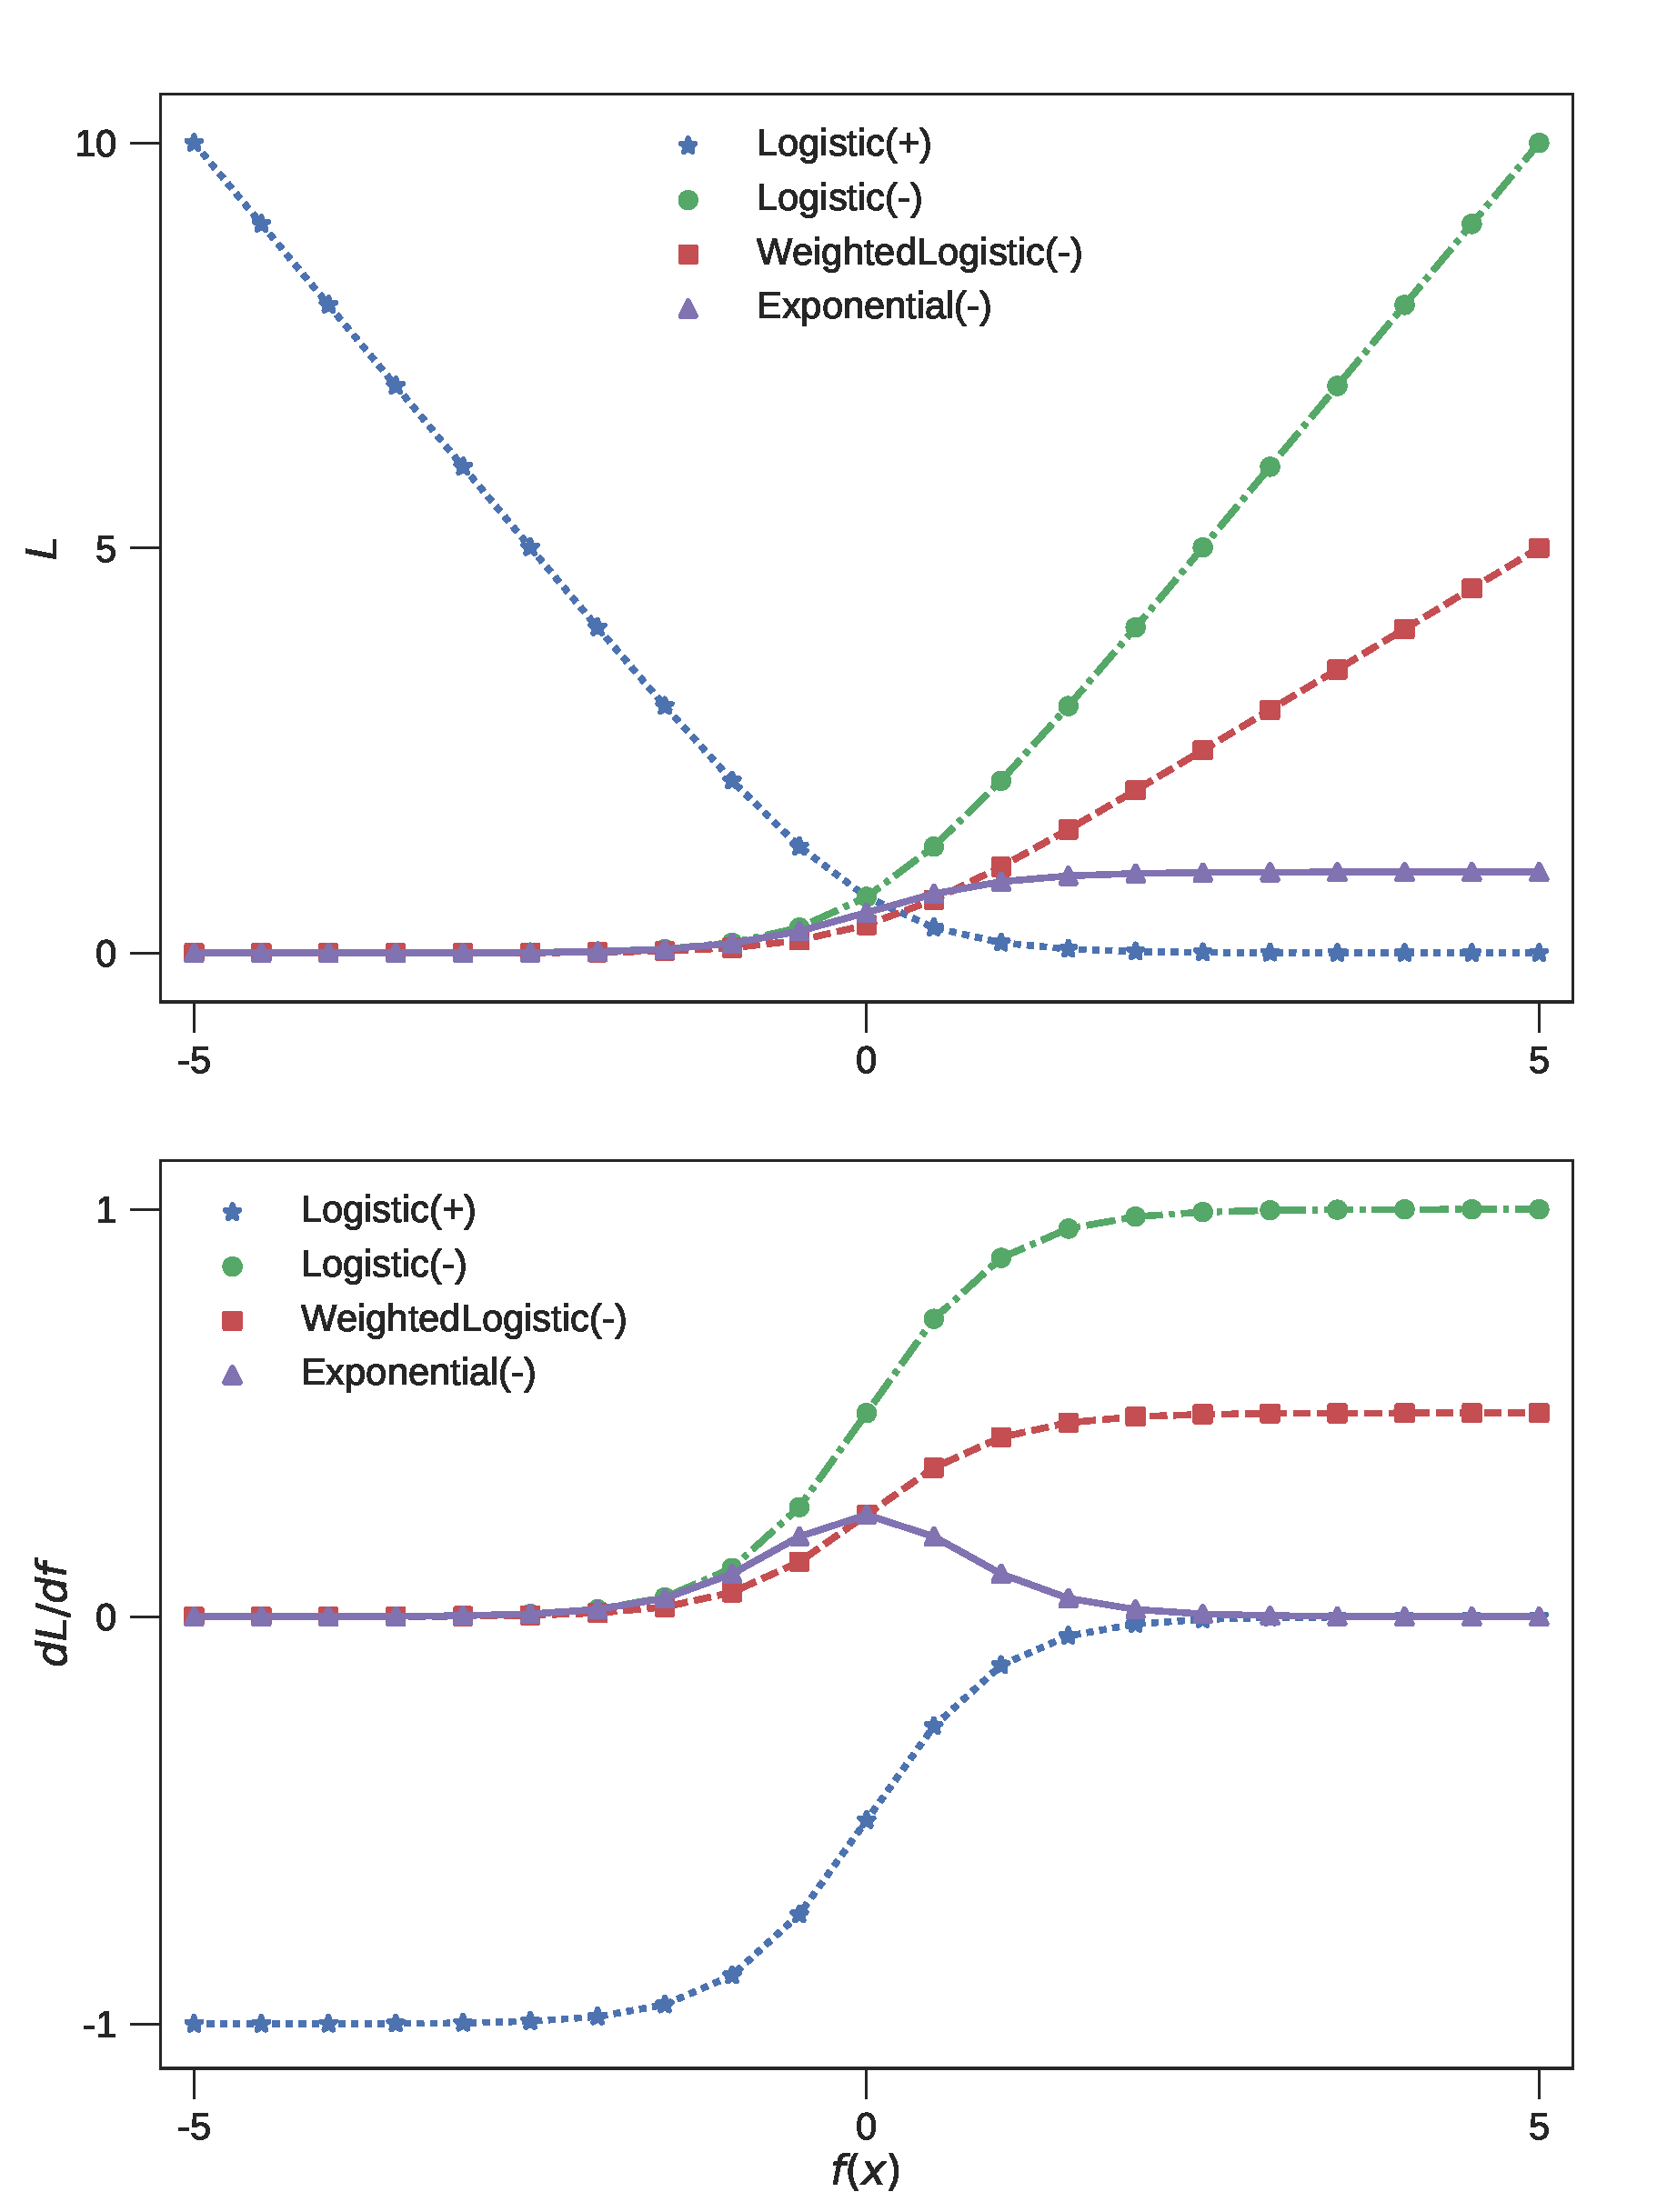
\includegraphics[width=1.05\linewidth]{img/losses}
\caption{
The differences in losses (top figure) and derivatives (bottom figure) with repect to the model output $f$ between the weighted logistic loss and the sigmoid loss for the negative class.
The \textbf{+} sign represents the loss of positive samples and the \textbf{-} sign stands for the loss of negative samples.
The sigmoid loss of negative examples reaches a plataeu and the derivative drops to zero in the very positive region.
The weighted logistic loss for negative is a linearly scaled logistic loss.
}
\label{fig:losses}
\end{figure}

%%%%%%%%%%%%%%%%%%%%%%%%%%%%%%%%%%%%%%%%%%%%%%%%%%%%%%%%%%%%%%%%%%%%%%
%%%%%%%% TEXT PU Learning setup
%%%%%%%%%%%%%%%%%%%%%%%%%%%%%%%%%%%%%%%%%%%%%%%%%%%%%%%%%%%%%%%%%%%%%%

\paragraph{PU Learning}

A training set for the positive and negative (PU) learning problems contains only a set of positive examples (P set) and a set of unlabeled samples (U set).
Unlabeled examples can be either positive or negative, meaning that there is no reliable negative examples available
One straightforward way to generate negative examples for training is to treat all the unlabeled examples as a set of negative examples with noises.
The problem then converts to learning with clean positive labels and noisy negative labels.
The goal of solving a PU learning problem is to learn a classifier that predicts as many positives as possible while keeping the false positive rate low, regardless the influence of false negative labels.
In other words, the purpose is to achieve high recall without sacrificing too much precision.


%%%%%%%%%%%%%%%%%%%%%%%%%%%%%%%%%%%%%%%%%%%%%%%%%%%%%%%%%%%%%%%%%%%%%%
%%%%%%%% TEXT Weighted loss for negatives
%%%%%%%%%%%%%%%%%%%%%%%%%%%%%%%%%%%%%%%%%%%%%%%%%%%%%%%%%%%%%%%%%%%%%%

\paragraph{Weighted logistic loss}

The mislabeled negative samples bias the classifier to have low recall.
It is possible to balance precision and recall by simply weighing the positive and negative examples differently, namely, let the positive and negative examples have different rates of contribution to the total loss.
Suppose a logistic loss is used, the corresponding weighted loss for a input-output pair $(x, y)$ for a classifier determined by parameters $\theta$ is:
\[
  l(x, y; \theta) =
    \begin{cases}
      - \alpha \log P(y=+1 \vert x; \theta), & y = +1 \\
      - \beta \log P(y=-1 \vert x; \theta), & y = -1
    \end{cases}
\]
where $\alpha$ and $\beta$ are weights for positive and negative class respectively, and $P(y\vert x; \theta)=\sigma(f(x; \theta))$ is the probablistic predictions by model $f(\cdot)$, activated by the sigmoid function $\sigma(\cdot)$.
This loss is referred to as the \textbf{weighted loss} in the rest of paper.
Empirically, the choice of $p$, $q$ can be made based on the highest precision and recall achieved on a validation set, or alternatively based on a class priors estimation\cite{du2014class}.
% Alternatively, one can also roughly assign $q=p(y=-1 \vert \tilde{y}=-1)$.
% This turns out to be part of the backward corrected loss proposed in  \cite{patrini2016making}:
% \begin{equation*}
%   \begin{aligned}
%     l_{\tilde{y_i}=-1} = - p(y_i=-1 \vert \tilde{y_i}=-1) \log p(y_i=-1 \vert x_i) \\ - p(y_i=+1 \vert \tilde{y_i}=-1) \log p(y_i=+1 \vert x_i)
%   \end{aligned}
% \end{equation*}
% % $$p( \tilde{y} \vert x, y) = \sum_{y}p(\tilde{y} \vert y)p(y \vert x)$$
% % $$p(y=+1 \vert \tilde{y}=+1) = 1 $$
% % $$p(y=-1 \vert \tilde{y}=+1) = 0 $$
% with $p(y_i=-1 \vert \tilde{y_i}=-1) = q$ and $p(y_i=+1 \vert \tilde{y_i}=-1) = 1-q$.



%%%%%%%% TEXT sigmoid Negative loss
\paragraph{Sigmoid Loss for the negative class}

As motivated in Section \ref{sec:related}, we used a class-dependent loss to down-weight the loss contribution of very positive predictions negative labels and still making full use of the clean positive labels.
The loss of positive examples is still a normal logistic loss and the loss of negative examples is replaced with a sigmoid loss \cite{tax2016class}:
\[
  l(x, y; \theta) =
    \begin{cases}
      - \log P(y=+1 \vert x; \theta), & y = +1 \\
      1 - P(y=-1 \vert x; \theta), & y = -1
    \end{cases}
\]
We called this class-dependent loss \textbf{sigmoid loss} in a sense it uses a sigmoid function as the loss of negative samples.
Using the logistic loss for the positive class and the sigmoid loss for the negative class is an interpretation of the prior knowledge that the positive labels are reliable whereas the negative labels are not.

Figure \ref{fig:losses} shows the differences in losses and derivatives with respect to model output between weighted logistic loss and sigmoid loss.
The main feature of sigmoid loss for negative examples is its small changes in the region of confident positive, compared to the weighted loss with $\alpha=1$ and $\beta=0.5$.
As a consequence, the corresponding derivative decreases to zero as the model prediction increases in the positive direction.


%%%%%%%% TEXT Bootstrapping
\paragraph{Hard bootstrapping loss for the negative class}
In addition to the proposed sigmoid loss, we also modify the hard bootstrapping loss by Reed et al. \cite{reed2014training} for PU learning to set a benchmark.
The modified class-dependent hard bootstrapping loss a pair of inputs and label $(x,y)$ is:
% $$l_- = - \beta \log p(y=-1 \vert x) - (1-\beta) \sum_{j\in \{-1, +1\}} p(y=j \vert x) \log p(y=j \vert x)$$
\begin{equation*}
\resizebox{\columnwidth}{!}{$
  l(x, y; \theta) =
    \begin{cases}
      - \log P(y=+1 \vert x; \theta), & y = +1 \\
      - \beta \log P(y=-1 \vert x;\theta) - (1-\beta) \log P(y=\hat{y} \vert x;\theta), & y = -1
    \end{cases}
$}
\end{equation*}
where $\hat{y} = \argmax_{j\in\{-1,+1\}}{P(y=j \vert x)}$ is the class with the highest predicted probability and $0<\beta<1$.
The first term of the objective is a weighted logistic loss and the second term can be considered as a regularization term to encourage consistent predictions.
This loss is referred as \textbf{bootstrapping loss} for the rest of this paper.
% \begin{equation*}
%   \begin{aligned}
%     H = - \sum_{j\in\{-1,+1\}} p(y_i=j \vert x_i) \log p(y_i=j \vert x_i) \\
%     \sim - \sum_{j\in\{-1,+1\}} \delta(y_i - \hat{y_i}) \log p(y_i=j \vert x_i)
%   \end{aligned}
% \end{equation*}
% which intuitively encourages the model to make confident predictions \cite{grandvalet2005semi}.

%%%%%%%% TEXT Segmentation
\paragraph{Extending PU learning from classification to segmentation}
In Section \ref{introduction}, we argue that learning with unlabeled foreground pixels is similar to a PU learning setup.
Howvever, there is still differences between learning with unlabeled foreground pixels and learning with positive and unlabeled examples.

The first difference is that each example in the normal PU learning setup is independent of each other, whereas pixels in images are not.
Assuming the probability of mislabeling foreground pixel as the background is independent of its neighbor pixels, the classification losses can be applied to segmentation problems by performing per-pixel classification problems.

Another difference between incomplete segmentation and a normal positive and unlabeled learning problem is that pixels for objects of various categories can be unlabeled.
Supposing there are $K$ categories of interest, varying from class $1$ to class $K$, the class $0$ is for unlabeled data which may or may not belong to the $K$ defined categories.
The sigmoid loss can be extended train deep learning models with unlabeled examples from various categories:

\[
  l(x, y; \theta) =
    \begin{cases}
      - \alpha_1 \log P(y=1 \vert x; \theta), & y = 1 \\
                                              & \vdots \\
      - \alpha_K \log P(y=K \vert x; \theta), & y = K \\
      \beta (1 - P(y=0 \vert x; \theta)), & y = 0
    \end{cases}
\]
where $\alpha_1, \dots, \alpha_K, \beta$ are weighting factors, and $P(y \vert x; \theta)$ is the predictied probability for class $y$, i.e., model output activated by the softmax function.
This loss is referred to as the \textbf{softmax loss} because it uses a softmax activation for the model output.

% Similar modifications can be made to the cross-entropy loss, namely, keeping the losses for classes $1$ to $K$ unchanged and applying the loss for negative class to the loss for class 0, supposing there are $K$ positive classes and one negative class.
% Alternatively, one can apply a one-vs-all strategy, with which the normal logistic loss is used for positive classes while the weighted, sigmoid and bootstrapping loss can be used for the negative class.

%%%%%%%% TEXT Expontial loss FADE IN
\paragraph{Implementation details}
We introduced the sigmoid loss only after training with a class-weighted cross entropy loss for a few epochs.
The sigmoid loss of negative examples saturates for very positive outputs, meaning that the confident, positive prediction has little contribution to the weights update.
The wrong confident predictions can introduce problems at the beginning of the training procedure when the confident predictions are likely to be made at random.
Otimization would reach the plateau when the model made all positive predictions with high confidence.
Besides, we also introduce the modified hard bootstrapping loss only after a few epochs trained with class-weighted loss because it also relies on a nonrandom model for sufficiently reliable prediction $\hat{y}$.


%%%%%%%% TEXT Imbalanced

Another problem encountered in the PU learning setup is the class imbalance introduced by negatively labeled positive samples.
A balanced dataset can become imbalanced in the presence of false negative labels, especially if only a small portion of positive samples are correctly labeled.
We reweighed positive and negative samples based on their occurrences of the observed labels to alleviate the influence of imbalance for training.
Note that the class-weighted logistic loss reweighed the classes in addition to this frequency balancing class weight.


\section{Experiments}
\label{sec:experiments}

\subsection{The influence of synthesized segmention noises on feature transferability}
\label{subsec:robustness}

%%%%%%%% TEXT Experiment setup

\paragraph{Experiment setup}

To investigate the influence of inexhaustive segmentations, misclassifications and false segmentations on feature transferability, we set up experiments with synthesized label noises from a well-annotated dataset, the PASCAL VOC2011 segmentation dataset\cite{everingham2015pascal}.
Fifteen out of twenty categories of the VOC2011 dataset were selected to form a \textit{pre-training dataset} and the other categories formed a \textit{fine-tuning dataset}.
The pre-training dataset was used to train a Fully Convolutional Network with AlexNet (FCN-AlexNet) model\cite{long2015fully} for segmentation in the presence or absence of synthesized segmentation errors.
The fine-tuning dataset was used to fine-tune the weights of convolutional layers from the pre-trained FCN-AlexNet models.
Inexhaustive segmentations, misclassifications, and false segmentations were synthesized separately with stochastical corruptions to the well-annotated pre-training dataset, followed the descriptions in Section \ref{subsec:formulation}.
Fine-tuned models were evaluated by mean intersection over union ratio (mean IU) achieved on the fine-tuning test set, referring to as the \textit{fine-tuning performance}.
Performance improvement of fine-tuning transferred models compared to an randomly initialized model indicates the transferability of pre-trained weights.

\paragraph{Experiment details}

To avoid that the choice of pre-training and fine-tuning splitting for categories influence the results, the 20 categories of VOC2011 were divided equally into four folds.
Each fold was studied separately, and the exact partitions of each fold are listed in Table \ref{tab:robustness}.
The training dataset was enriched with extra segmentations by Hariharan et al.\cite{hariharan2011semantic}
To keep the segmentation task simple, we used only single-object images, resulting in totally 4000 training images for 20 categories available for pre-training, fine-tuning and evaluation.
In order to accelerate the training process, we subsampled the original images by four times.
Fully Convolutional Networks with AlexNet was used for experiments because of its relatively small capacity and thus short training time.
The existence of an ImageNet model for AlexNet can be beneficial to set a performance reference.
The non-transferred layers were randomly initialized with Xavier Initialization.
The ImageNet model and completely random weight initialization were considered as the upper bound and lower bound, respectively, for various pre-trained weights summarized in Table \ref{tab:robustness}.
The default hyperparameters of FCN-AlexNet in \cite{long2015fully} were kept unchanged.
Training run 240,000 iterations for pre-training phase, and 12,000 iterations for fine-tuning phase.
Snapshots for trained models were taken every 4,000 iterations.
Each experiment was repeated three times, mean and standard deviation were computed over the last five snapshots for all repetitions.


% \noindent \textit{What Table \ref{tab:robustness} tell us.
% How annotation errors were synthesized;
% How synthesizations are different from reality;
% Transferability of noisy models compared to clean models.
% }


\paragraph{Inexaustive Segmentation}

Fine-tuning performances of transferring models pre-trained with complete labels and half of the objects unsegmented respectively are summarized in Table \ref{tab:robustness}.
The HalfUnsegmented model transferred into a fine-tuned model with an average mean IU 0.04 worse than the CompleteLabels model, almost the same as training a model with random weight initialization.
This result indicates that inexhaustive segmentation can have a negative impact on weights transferability.
By applying the sigmoidal negative loss to pre-train models with half of the objects segmented, we were able to achieve a comparable fine-tuning performance as using the complete segmentation to pre-train.
% The details of implementing sigmoidal negative loss for the pre-training dataset will be discussed in Section \ref{subsec:pulearning}.

\paragraph{Misclassifications}

Models pre-trained with random labels are listed in Table \ref{tab:robustness}.
Compared to the CompleteLabels model (the one trained with true labels), both the model trained with all random labels or half true half random labels led to worse fine-tuning performances.
Fine-tuned performances of the AllRandomLabels model and the HalfRandomLabels model were no better than randomly initializing model weights, indicating poor weights transferability of a trained model in the presence of random labels to segmentations.
In other words, misclassification noises in segmentation can impact the transferability of convolutional weights negatively.

However, binarizing labels for pre-training was able to achieve equivalent fine-tuning performance as using true labels.
It achieved better performance than training to segment the exact classes but with random labels.
Binarized labels are accurate but imprecise because pixel labels were randomized among foreground classes and binarizing labels lead to correct segmentation for foreground and background.
This observation indicates that inaccurate labels may have more significant negative influence than imprecise labels for feature transferability.

Additionally, we studied the influence of categorizing classes for pre-training to keep the labels precise to some extent.
We categorized the fifteen classes in the pre-training set into person, animal, vehicle, indoor according to \cite{everingham2015pascal} and trained a model to transfer, shown as the error bars on lines in figure \ref{fig:categories} at categories 4.
As a comparison, the fifteen classes were also randomly categorized into 4, 7, 11 categories and shown as isolated error bars in figure \ref{fig:categories} at categories 4, 7, 11 respectively.
Figure \ref{fig:categories} shows that categorizing pre-training classes had little effect to the fine-tuning performance of transferred models.
Even categorizing classes at random without explicit meaning could pre-train weights better than random initialization (shown as error bar at categories 0).
It can be beneficial to binarize or group classes into hyper-categories to learn better transferable weights in the presence of misclassifications.

\paragraph{False segmentations}

To synthesize false segmentations, we selected one category, either cat or dog depending on the folds, as the target category and all the other 14 categories in the pre-training dataset became non-target, as discussed in Section \ref{subsec:formulation}.
In the presence of false segmentations, instances from non-target categories can be misannotated as the target category with a probability of $p_{10}= 0.5$.
The result pre-trained models is named as FalseSegmentHalf in Table \ref{tab:robustness} respectively.
The noise-free counterpart of is the model pre-trained with segmentations of the selected target category only and the other 14 categories remained unsegmented, denoted as NoFalseSegmented.

Compared to the NoFalseSegmentated model, transferring the HalfFalseSegmented model introduced no significant decrease in fine-tuning performance.
This observation indicates that false segmented meaningful objects may have a little negative impact when they are used for pre-training transferable weights.



\begin{table*}[t]
\resizebox{\textwidth}{!}{
\centering
\begin{tabular}{l|l|llll|l}

\hline
                                                                                      & \begin{tabular}[c]{@{}c@{}}Initial Feature\\ Extractor\end{tabular} & \multicolumn{4}{c|}{Fine-tuning mean IU per pretraining-finetuning fold}                                                                                                                                                                                                                                                                                                                                                                     & \multicolumn{1}{l}{\multirow{2}{*}{\begin{tabular}[c]{@{}l@{}}Average \\ mean IU\\ across \\ four folds\end{tabular}}} \\ \cline{1-6}
\begin{tabular}[c]{@{}l@{}}Fine-tuning\\ categories\end{tabular}                      &                                                                     & \multicolumn{1}{l}{\begin{tabular}[c]{@{}l@{}}aeroplane, \\ bicycle, bird,\\ boat, bottle\end{tabular}} & \multicolumn{1}{l}{\begin{tabular}[c]{@{}l@{}}bus, car, \\ cat, \\ chair, cow\end{tabular}} & \multicolumn{1}{l}{\begin{tabular}[c]{@{}l@{}}dining table,\\ dog, horse, \\ motorbike,\\ person\end{tabular}} & \multicolumn{1}{l|}{\begin{tabular}[c]{@{}l@{}}potted plant, \\ sheep, sofa, \\ train, TV\end{tabular}} & \multicolumn{1}{l}{}                                                                                                   \\ \hline
\multirow{2}{*}{\begin{tabular}[c]{@{}l@{}}Upper bound \&\\ lower bound\end{tabular}} & ImageNetModel                                                       & $0.42\pm0.01$                                                                                           & $0.51\pm0.01$                                                                               & $0.49\pm0.01$                                                                                                  & $0.47\pm0.01$                                                                                           & $0.47\pm0.01$                                                                                                          \\
                                                                                      & RandomWeights                                                       & $0.29\pm0.01$                                                                                           & $0.29\pm0.03$                                                                               & $0.27\pm0.01$                                                                                                  & $0.30\pm0.02$                                                                                           & $0.29\pm0.02$                                                                                                          \\ \hline
\multirow{3}{*}{\begin{tabular}[c]{@{}l@{}}Inexaustive \\ Segmention\end{tabular}}    & CompleteLabels                                                      & $0.29\pm0.01$                                                                                           & $0.36\pm0.01$                                                                               & $0.29\pm0.01$                                                                                                  & $0.37\pm0.01$                                                                                           & $\mathbf{0.33\pm0.01}$                                                                                                 \\
                                                                                      & HalfUnsegmented                                                     & $0.26\pm0.01$                                                                                           & $0.30\pm0.03$                                                                               & $0.28\pm0.03$                                                                                                  & $0.32\pm0.02$                                                                                           & $0.29\pm0.02$                                                                                                          \\
                                                                                      & SigmoidalLoss                                                       & \multicolumn{1}{l}{$0.30\pm0.01$}                                                                       & \multicolumn{1}{l}{$0.37\pm0.01$}                                                           & \multicolumn{1}{l}{$0.31\pm0.02$}                                                                              & \multicolumn{1}{l|}{$0.34\pm0.02$}                                                                      & $\mathbf{0.33\pm0.02}$                                                                                                 \\ \hline
\multirow{3}{*}{Misclassification}                                                    & AllRandomLabels                                                     & $0.29\pm0.01$                                                                                           & $0.33\pm0.03$                                                                               & $0.26\pm0.01$                                                                                                  & $0.28\pm0.01$                                                                                           & $0.29\pm0.01$                                                                                                          \\
                                                                                      & HalfRandomLabels                                                    & $0.27\pm0.01$                                                                                           & $0.33\pm0.02$                                                                               & $0.25\pm0.01$                                                                                                  & $0.29\pm0.01$                                                                                           & $0.29\pm0.01$                                                                                                          \\
                                                                                      & BinarizedLabels                                                     & $0.30\pm0.02$                                                                                           & $0.35\pm0.01$                                                                               & $0.29\pm0.02$                                                                                                  & $0.35\pm0.03$                                                                                           & $\mathbf{0.32\pm0.02}$                                                                                                 \\ \hline
\multirow{2}{*}{\begin{tabular}[c]{@{}l@{}}False \\ Segmentaion\end{tabular}}         & NoFalseSegmented                                                    & $0.26\pm0.01$                                                                                           & $0.37\pm0.03$                                                                               & $0.27\pm0.01$                                                                                                  & $0.33\pm0.04$                                                                                           & $\mathbf{0.31\pm0.02}$                                                                                                 \\
                                                                                      & FalseSegmentedHalf                                                  & \multicolumn{1}{l}{$0.27\pm0.01$}                                                                       & \multicolumn{1}{l}{$0.34\pm0.01$}                                                           & \multicolumn{1}{l}{$0.30\pm0.01$}                                                                              & \multicolumn{1}{l|}{$0.32\pm0.01$}                                                                      & $\mathbf{0.31\pm0.01}$                                                                                                 \\ \hline

\end{tabular}
}
\caption{
Segmentation performance for FCN-AlexNet models pre-trained with 15 categories from the PASCAL VOC2011 dataset and fine-tuned with the other 5 categories.
\textbf{ImageNetModel} represents the pre-trained ImageNet model (upper bound);
\textbf{RandomWeights} indicates that the randomly initialized weights (lower bound);
All the other extractors were pre-trained in the presence or absence of the corresponding label noises listed in the leftmost column.
Half of the objects unsegmented result in pre-trained models not significantly better than random weight initialization.
Introducing the sigmoidal negative loss in the pre-training phase was able to improve the fine-tuning performance to be comparable to pre-trained model with complete segmentations.
Random labels interfered the fine-tuning performance of transferred models and binarizing classes as foreground and background for in the pre-training dataset help overcome the negative effects of random labels.
Including false segmentations had little influence on transferred models.
% \textit{SingleCategory} was pre-trained on only one annotated category, either ``dog'' or ``cat'' depending on the fold, and the other categories were left unannotated;
% \textit{BinaryLabels} was pre-trained with binary labels that any objects of the fifteen categories were annotated as one single category, namely ``dog'' or ``cat'' depending on fold;
% \textit{TrueLabels} was pre-trained with all objects segmented and assigned to 15 categories correctly;
% \textit{AllRandomLabels} was pre-trained with all objects correctly segmented but assigned random labels;
% \textit{HalfRandomLabels} was pre-trained with all objects correctly segmented and half of them randomly assigned labels;
% \textit{IncompleteLabels} was trained with datasets that objects were annotated correctly with a probability of 0.5;
}
\label{tab:robustness}
\end{table*}


%%%%%%%% Figure categorizing classes
\begin{figure}[t]
\centering
   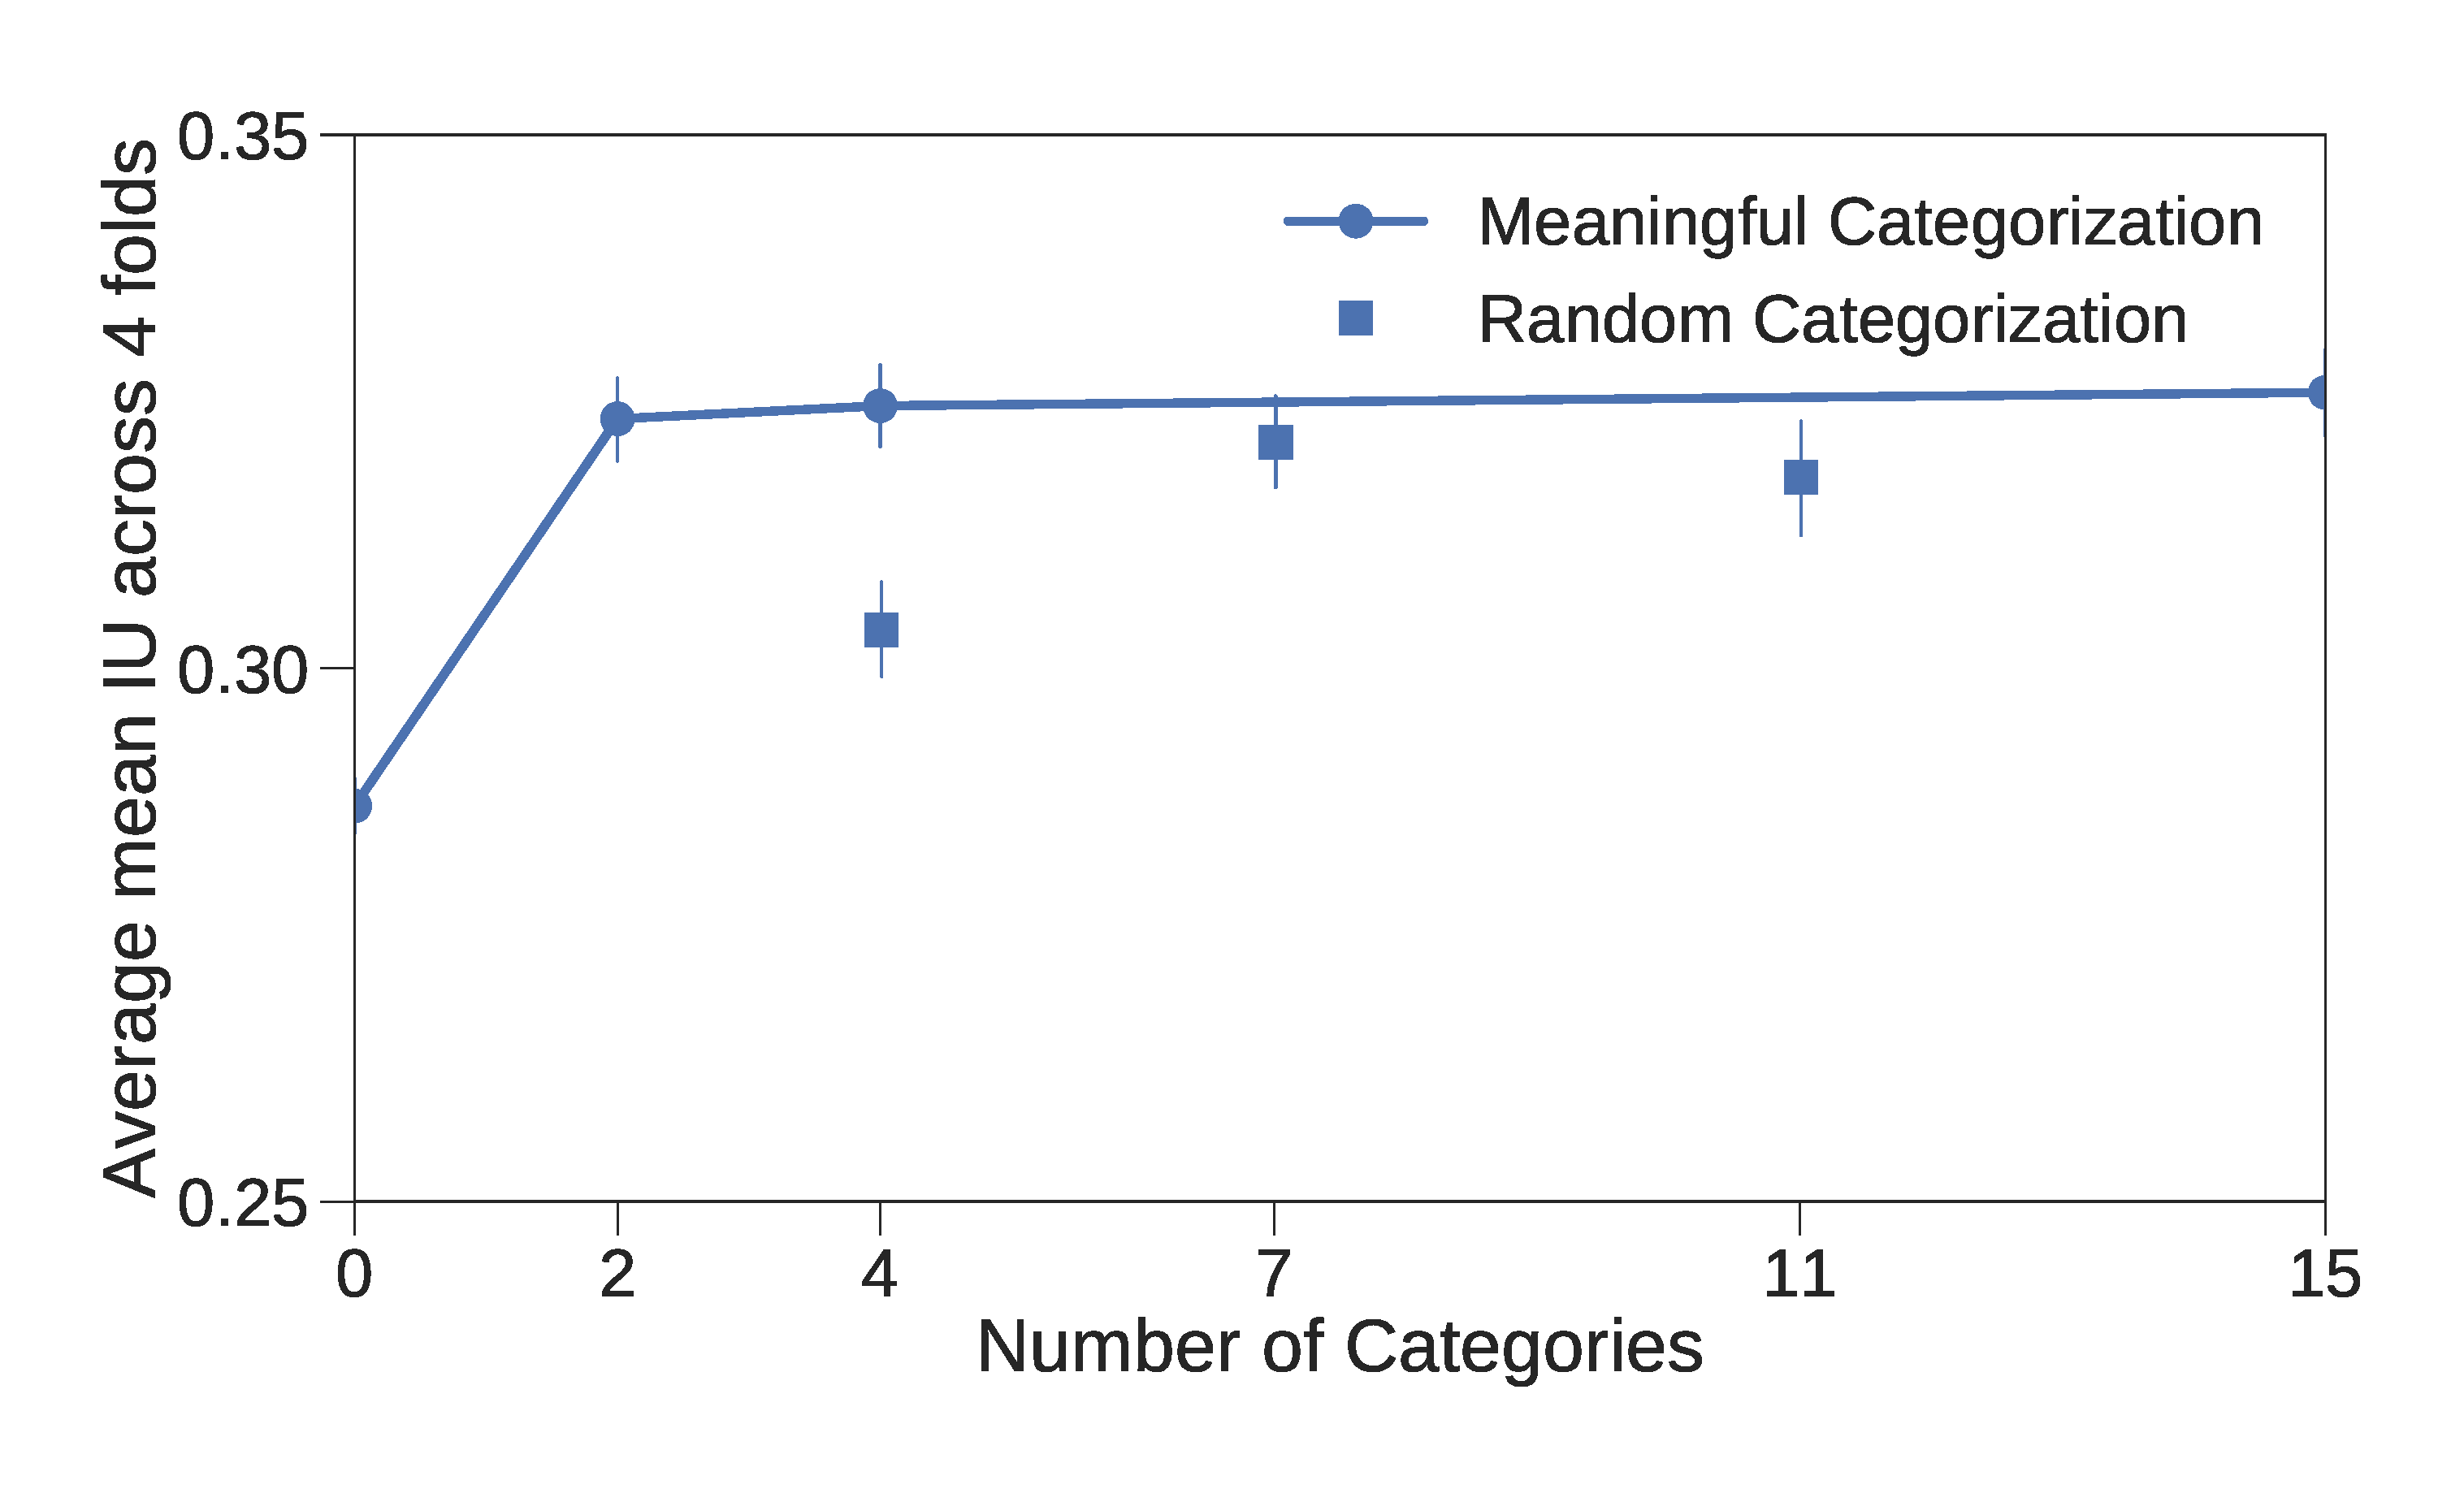
\includegraphics[width=1.\linewidth]{img/num_classes.eps}
\caption{
Test performance for models fine-tuned from pre-trained weights using data of categorized pre-training classes.
Isolated error bars denote random categorizations (RC) of the 15 classes, while error bars located on lines denote the meaningful categorization.
Zero categorize means no pre-trained weights used and the model was random initialized.
The displayed mean IU/mean accuracies and standard deviations were averaged over four folds listed in Table \ref{tab:robustness}.
The trend shows that binarizing and categorizing classes had little negative effect on feature transferability.
}
\label{fig:categories}
\end{figure}


%%%%%%%%%%%%%%%%%%%%%%%%%%%%%%%%%%%%%%%%%%%%%%%%%%%%%%%%%%%%
%%%%%%%%%% PU Learning
%%%%%%%%%%%%%%%%%%%%%%%%%%%%%%%%%%%%%%%%%%%%%%%%%%%%%%%%%%%%

\subsection{Learn to classify with positive and unlabeled samples}
\label{subsec:pulearning}


\paragraph{2-dimensional moons dataset}

Figure \ref{fig:moons} shows the decision boundaries of a 2-layer multilayer perceptron, with 6 neurons per layer, trained with the weighted loss, the sigmoidal loss and the bootstrapping loss.
Four hundred samples per class were drawn randomly from two interleaving half circles with noises added with a minor standard deviation.
The leftmost column in the figure shows the multilayer perceptron trained with complete positive labels and the normal logistic loss while the other three columns show the classifier trained with half of the positive examples labeled as negative.
For sigmoidal negative loss, the mislabeled positive examples faraway from the decision boundary have smaller derivatives the ones closer to but still distant from the decision boundary.
As a consequence, optimization performed as counting the weights update contributions differently for confident and unconfident prediction instead of simply decreasing the overall estimation for the negative loss.
The result decision boundary becomes more distant from the positive cluster, and confident predictions are made in more areas of the space.
% The positive examples push the decision boundary away from the positive cluster while negative examples closed to the decision boundary instead of those away from the decision boundary pull the decision boundary towards the positive cluster.

%%%%%%%% FIGURE MOONS

\begin{figure*}
\begin{center}
% \fbox{\rule{0pt}{2in} \rule{.9\linewidth}{0pt}}
   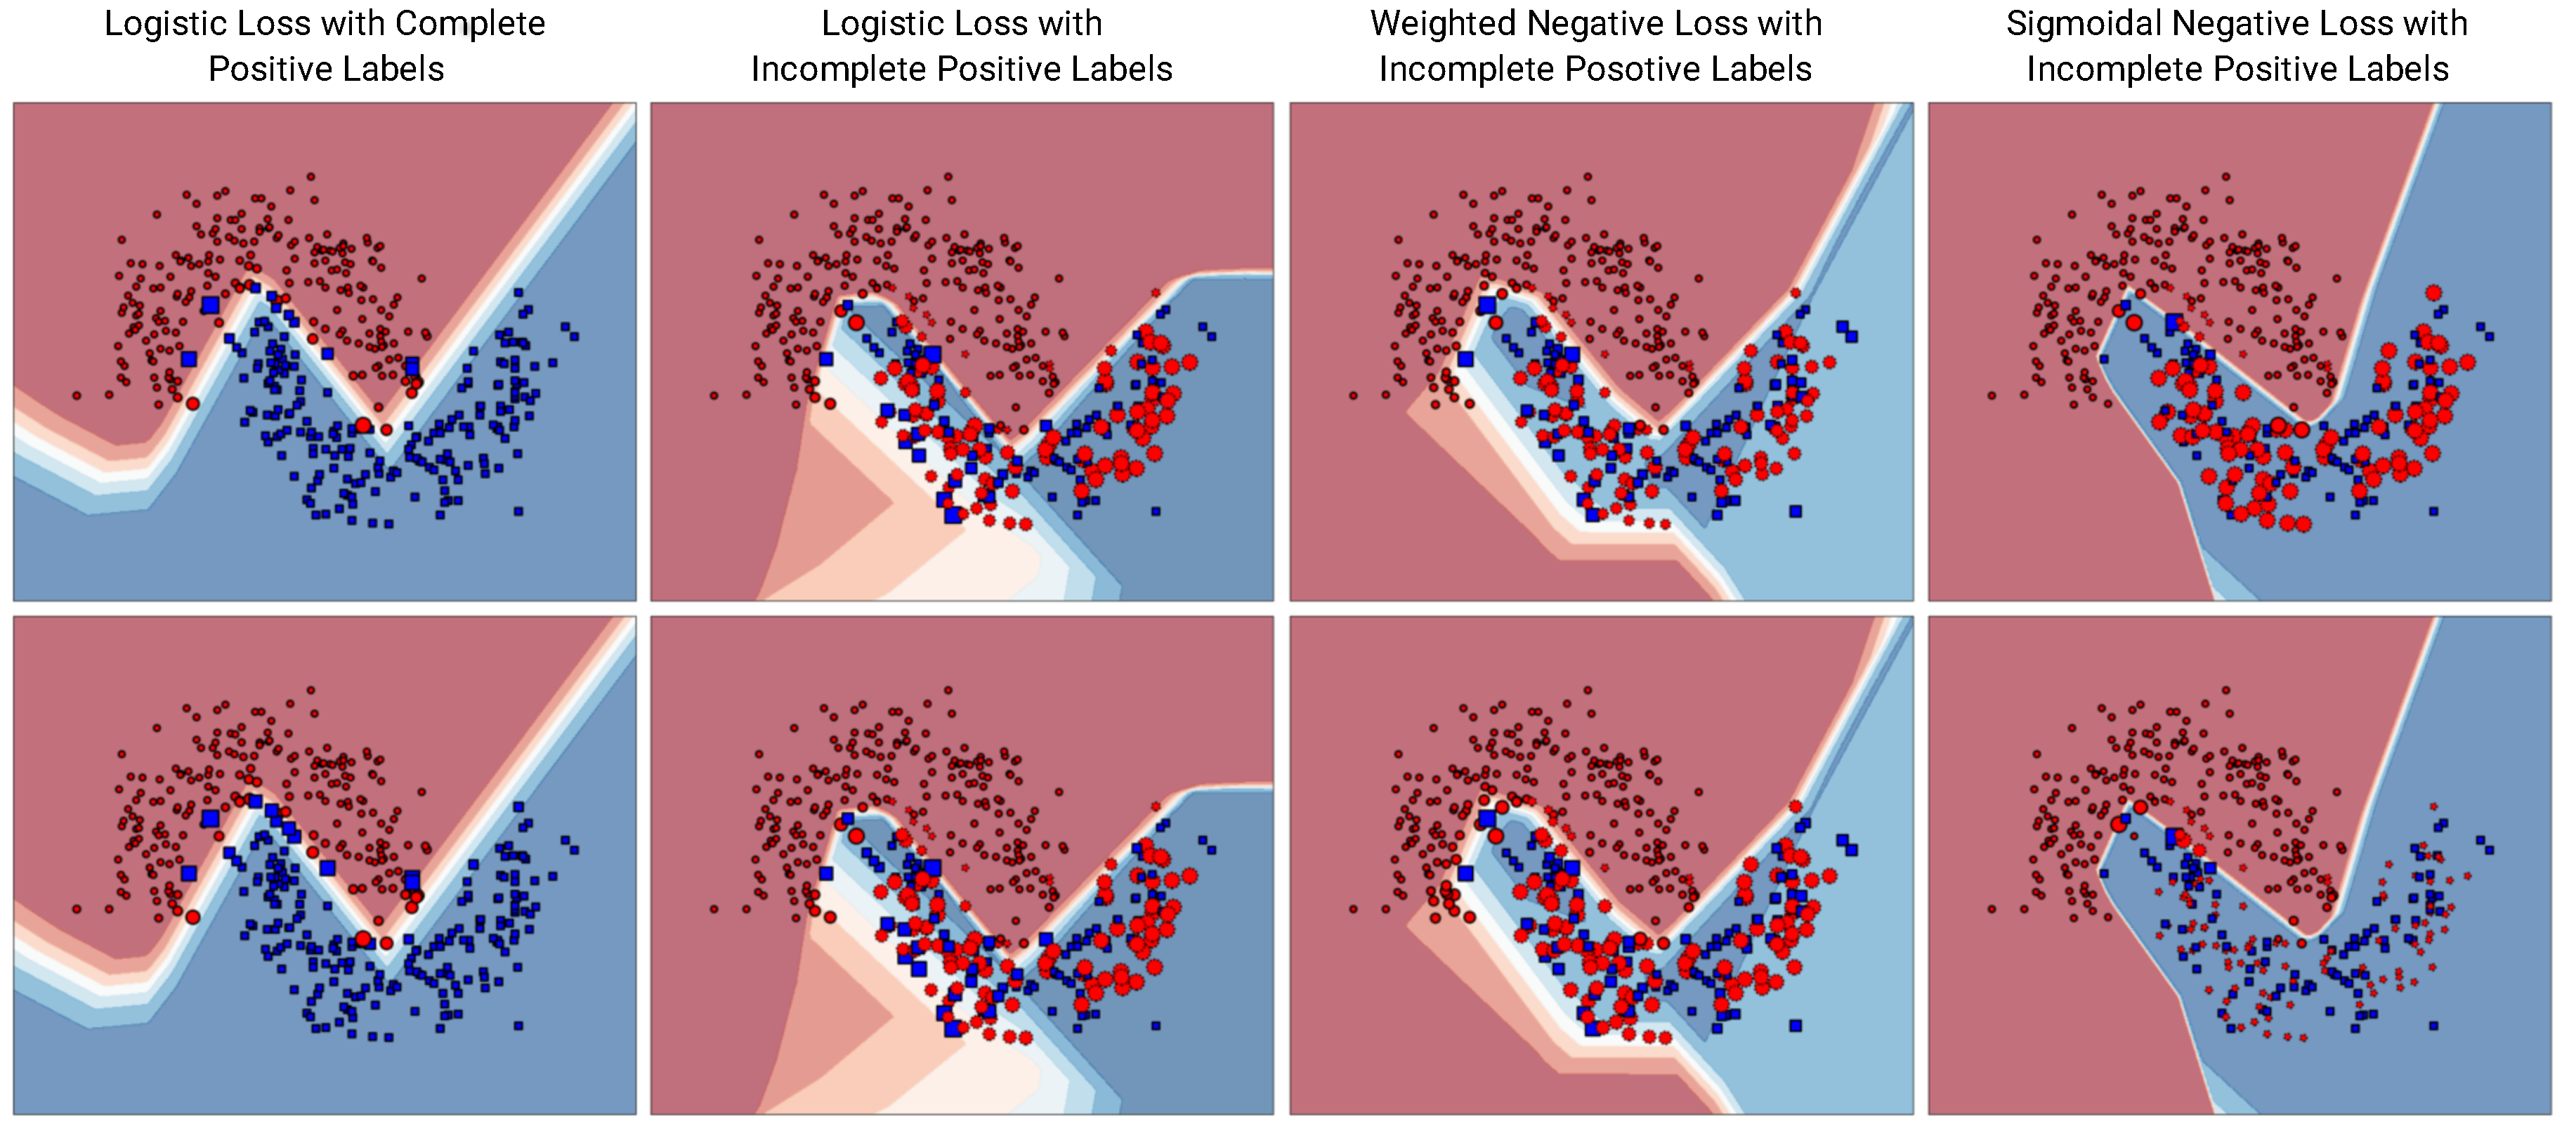
\includegraphics[width=0.95\linewidth]{img/moons}
\end{center}
   \caption{
   Decision boundaries, optimal losses, and derivatives of a 2-layer multilayer perceptron trained with different losses on a 2D moons dataset with the unlabeled positive.
   The \textbf{top row} demonstrates the per-class normalized training losses with \textbf{markers sizes} and the \textbf{bottom row} displays the per-class normalized loss derivatives w.r.t the output with marker sizes.
  %  The \textbf{leftmost} figures have complete positive labels, meaning the positive and negative labels are all correct, whereas, in \textbf{the other figures} only half of the positives were correctly labeled and the rest were mixed with the negative samples.
   A \textbf{red circle} indicates an example labeled as positive and a \textbf{blue square} indicates the example has a negative label.
   The \textbf{background colors} represent the probability for the area to be positive given by the classifier trained with the given samples and labels: \textbf{red} for high probability areas, \textbf{blue} for low probability areas and \textbf{white} for the class transition areas, i.e.decision boundaries.
   Compared to the normal logistic loss and weighted logistic loss, the decision boundary optimized with sigmoidal negative loss is more distant from the positive cluster.
   The sigmoidal negative loss has saturated losses and low derivatives for predictions farther from the decision boundary.
   }
\label{fig:moons}
\end{figure*}

\paragraph{CIFAR dataset}

Images from the CIFAR10 dataset were used as positive (P) examples, and images from the CIFAR100 dataset were considered as the negative (N) examples.
We trained a CNN model to classify images into eleven classes: ten positive classes from CIFAR10 and a negative class for images from CIFAR100.
To synthesize a PU learning setup, we correctly labeled only part of positive images from CIFAR10 and the rest were assigned negative labels together with CIFAR100 images, forming the unlabeled (U) set.
An eight layer CNN model was trained with different choices of losses and with the labeled positive examples and unlabeled examples.
Model performances were then evaluated on a separate test set of combined CIFAR10 and CIFAR100 with true labels.

The architecture of the CNN model can be found in Appendix \ref{sec:support}.
Each model was trained from scratch with Adam optimizer and base learning rate 0.0001.
Experiments were repeated three times with random split of P set, and U set and standard deviations were around 0.01 if not explicitly mentioned.
Note that there is no category overlap between CIFAR10 dataset and CIFAR100 dataset.

%%%%%%%% TABLE CIFAR10 50%

Table \ref{tab:cifar} summarizes the test precisions and recalls of using different losses to learn with true positive labels and noisy negative labels, compared to training with the normal cross-entropy loss.
With 50\% of the positive example correctly labeled and the rest assigned negative labels, the normal cross-entropy loss led to an imbalanced model with high precision but low recall, and therefore with a low f1-score.
By reweighing the negative loss by a factor of 0.5, we were able to balance precision and recall and improve the resulting f1-score significantly.
Sigmoidal negative loss and hard bootstrapping loss were able to achieve even slightly better f1-scores than the weighted negative loss, though not as good as training with clean labels with the same number of positive examples.
It is noteworthy that the weighted negative loss and hard bootstrapping loss achieved more balanced precision and recall than the sigmoidal negative loss.
That is because the two former losses were weighted by classes frequency of observed labels, around 0.67 for the negative class and 2 for positive classes, whereas the sigmoidal negative loss was not.
Reweighing the sigmoidal negative loss by observed label frequencies would trade too much precision for recall (0.74 and 0.83 respectively), resulting in a worse f1-score than not reweighing losses.
The sigmoidal negative loss seems to be easier over-balancing with the same choice of class weights.
% Besides, the optimal precision and recall for sigmoidal negative loss seem more unstable which may relate to the nonconvex class-dependent loss.


\begin{table}[t]
\resizebox{\columnwidth}{!}{
\centering
\begin{tabular}{ll|llll}
Annotation  & Loss & acc. & mean prec. & mean rec. & mean $F_1$ \\
\hline
P+N         & CrossEntropyU.   & 0.87 & 0.88 & 0.82 & 0.85 \\
50\%(P+N)   & CrossEntropyU.   & 0.83 & 0.84 & 0.78 & 0.80 \\
50\%P+U     & CrossEntropyU.   & 0.66 & 0.94 & 0.38 & 0.49 \\
\hline
50\%P+U     & WeightedNeg.     & 0.78 & 0.75 & 0.75 & 0.76 \\
50\%P+U     & SigmoidalNeg.    & \textbf{0.81} & \textbf{0.85$\pm0.03$} & 0.72$\pm0.03$ & 0.77 \\
50\%P+U     & BootstrapHard    & 0.80 & 0.76 & \textbf{0.81} & \textbf{0.78} \\
\end{tabular}
}
\caption{
Overall accuracy, the average of precision, recall, and f1-score over classes on a test set of the CIFAR dataset with true labels.
CIFAR10 images were used as positive images (P), and CIFAR100 images were used as negative images (N).
The top columns summarize the upper bound, lower bound and reference for learning with positive and unlabeled examples.
\textbf{Upper bound} Model trained with the complete positive and negative labels;
\textbf{Reference} Model trained with 50\% of the positive and negative examples;
\textbf{Lower bound} Model trained with 50\% labeled positive examples and unlabeled examples;
The proposed losses should achieve as high recall as possible while keeping the precision high as well.
The modified hard bootstrap loss achieved the highest average f1-score with 50\% positive examples unlabeled.
}
\label{tab:cifar}
\end{table}


%%%%%%%% FIGURE Varying positive annotating percetage

By varying the percentage of labeled positive examples, we compared learning with the labeled positive examples and noisy negative examples with the three different losses as shown in Figure \ref{fig:pct_annotating}.
Similarly as a result at 50\% positive examples labeled, the sigmoidal negative loss and hard bootstrapping loss had only little improvement compared to the weighted negative loss.
The assumption we made for the sigmoidal negative loss was that the probability of a negative example being wrong is dependent on the confidence.
However, the synthesized mislabeled positive examples were distributed at random when we synthesized them, meaning that the probability for a negative label being wrong is independent of the underlying distribution of the inputs.
No matter where the decision boundary is, such uniformly distributed incorrect negative labels are independent of the prediction confidence.
Therefore, it is expected for the sigmoidal negative loss and bootstrapping loss to have similar performance as the weighted negative loss.

Figure \ref{fig:pct_annotating} also demonstrates that learning with a subset of reliable negative examples (PN setup) outperformed learning with positive and unlabeled examples (PU setup) for any percentage of labeled positives and any losses being used.
This result was expected because the PN setup delivers extra information about which images in the unlabeled set are negative.
The PU setup is therefore only relevant when it is impossible to easily construct a subset of negative examples from the unlabeled data.
Otherwise, training with true positive and negative labels, and potentially with semi-supervised learning, would be superior to training with positive and unlabeled examples only.

\begin{figure}[t]
\centering
   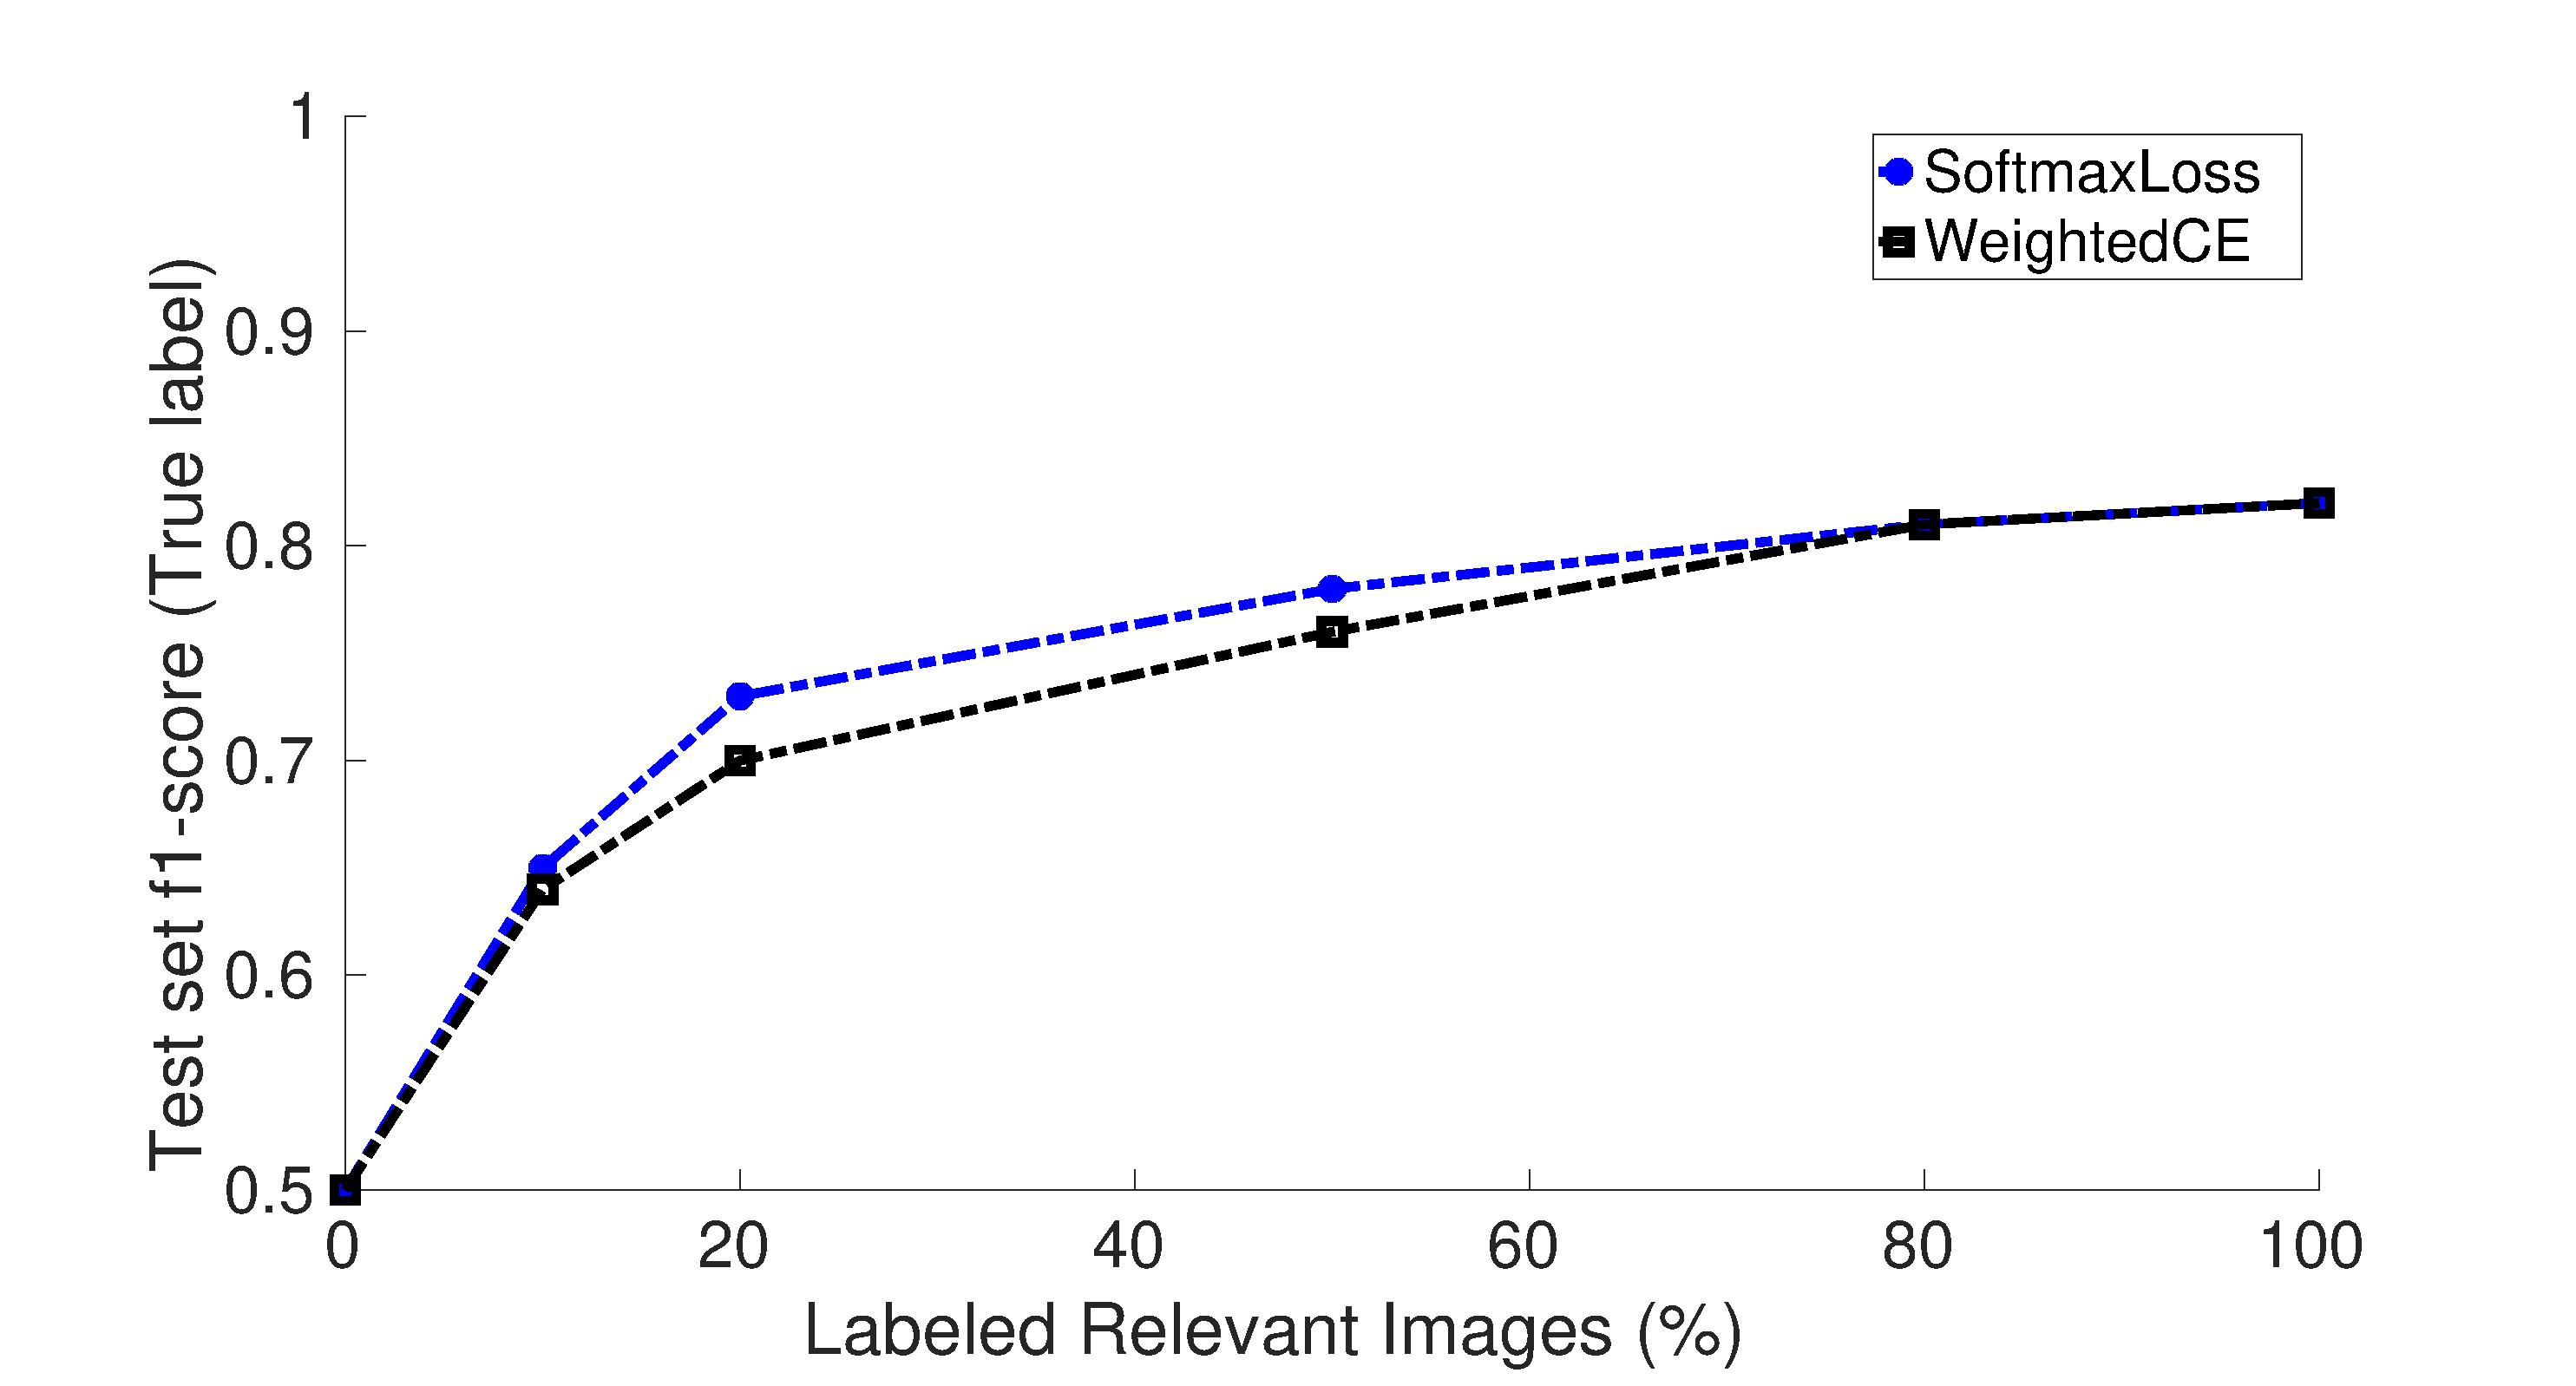
\includegraphics[width=1.05\linewidth]{img/pu_vs_pn}
\caption{
Comparing the f1-score achieved for weighted negative loss, sigmoidal loss and hard bootstrapping loss with varying percentage of labeled positive images
\textbf{P+N} represents training with the percentage of images with reliable positive and negative labels, and \textbf{P+U} stands for training with the positive (P) and unlabeled (U) sets.
The test performances of the three different losses did not show significant difference with the labeled positive percentage varying from 0\% to 100\%.
}
\label{fig:pct_annotating}
\end{figure}

%%%%%%%% Text Segmentation Pascal VOC2011
\paragraph{Pascal VOC2011 segmentation task}

To study the effect of sigmoidal negative loss on compensating incomplete segmentations, we used again the PASCAL VOC2011 dataset with extra segmentation\cite{hariharan2011semantic}.
We synthesized inexhaustive segmentations the same way as described in Section \ref{subsec:robustness}.
The same AlexNet-FCN model was trained together with the different loss functions for class 0 to predict binary segmentation, determining whether a pixel belongs to an object or not.
Only single-object images were used for training and testing to avoid the influence of two adjacent objects joining as one object because of binary segmentation.
The same hyperparameters for optimization were used as in Section \ref{subsec:robustness}.
The trained models were evaluated with the test set of PASCAL VOC2011 segmentation dataset with binary segmentations.

As shown in Table \ref{tab:pusegment}, the sigmoidal negative loss achieved the highest mean accuracy, approximately 0.07 better than training with the normal cross entropy loss.
In contrast to the improvement of mean accuracy, mean IU for models trained with either weighted negative loss or sigmoidal negative loss did not show significant improvement compared to the normal cross entropy loss.
The increase in the mean accuracy was caused by an increase in
foreground accuracy and a decrease in background accuracy.
In other words, the sigmoidal loss balances precision for recall, similarly as observed in training the CIFAR dataset.
The decrease in precision, however, can interfere the improvement mean IU since the mean IU counts for both low false positive rate and low false negative rate.

%%%%%%%% Text Fine-tuning performance with exponential loss

We then applied the sigmoidal negative loss to the pre-training phase of the experiment for inexhaustive segmentations in Section \ref{subsec:robustness}.
We were able to recover the negative influence of inexhaustive segmentations on the fine-tuning performance of the pre-trained models.
Note that we learned foreground/background segmentation instead of multi-class segmentation when applied the sigmoidal negative loss because we discovered binarizing pre-training classes had little effect to feature transferability in this experimental setup.
% {TODO} and the potential difficulty in extending sigmoidal negative loss to a multi-class scenario as we will discuss more in Section \ref{sec:discussion}.


%%%%%%%% TABLE Segmentation Pascal VOC2011
\begin{table}[t]
\resizebox{\columnwidth}{!}{
\centering
\begin{tabular}{ll|llll}
Annotation  & Loss & overall acc. & mean acc. & f.w. IU & mean IU \\
\hline
% Complete            & CrossEnt.U       &  0.88 & 0.60 & 0.48 & 0.80 \\
% 50\%Unsegmented     & CrossEnt.U       &  0.83 & 0.31 & 0.27 & 0.70 \\
% 50\%Unsegmented     & WeightedU        &  0.83 & 0.34 & 0.29 & 0.70 \\
% 50\%Unsegmented     & ExponentialU     &  0.83 & 0.34 & 0.29 & 0.70 \\
Complete       & CrossEntropy       &  0.90 & 0.85 & 0.82 & 0.75 \\
50\%Unseg.     & CrossEntropy       &  0.85 & 0.68 & 0.73 & 0.60 \\
50\%Unseg.     & WeightedNeg.       &  0.84 & 0.71 & 0.73 & \textbf{0.62} \\
50\%Unseg.     & SigmoidalNeg.      &  0.83 & \textbf{0.75} & 0.72 & \textbf{0.62} \\
\end{tabular}
}
\caption{
The best foreground/background segmentation performance achieved on the test set of PASCAL VOC2011 segmentation dataset with the normal cross entropy loss, weighted negative loss, and sigmoidal negative loss in the presence of inexhaustive segmentation.
A class weight of 0.7:1.75 was used to balance the sample frequency differences of the two classes.
The negative loss was further weighted by a factor of 0.5 for the weighted negative loss.
Mean accuracy is equivalent to the average recall over the two classes.
Mean IU is the average intersection over union ratio (IU) over two classes and f.w. IU is the frequency weighted average of IU over the two classes.
Experiments were repeated twice and standard deviations were approximately 0.02.
The sigmoidal negative loss achieved a better mean accuracy than weighted negative loss and a similar mean IU as the weighted negative loss.
Both losses performed better than the normal cross entropy loss in the presence of 50\% objects unsegmented.
}
\label{tab:pusegment}
\end{table}


%%%%%%%% Figure Segmentation Pascal VOC2011
Selective predictions made by models trained with the sigmoidal negative loss and the cross entropy loss were presented in Figure \ref{fig:pusegment}.
For these two example images, the model trained with the cross entropy loss failed to segment objects from images whereas sigmoidal negative loss predicted segmentations on the position of the objects.
The coarse outlines were mainly due to the limited compacity of the FCN-AlexNet model.
The third column shows predictions given by model trained with complete training segmentation, and it did not produce more accurate outlines.

\begin{figure}
\centering
  \begin{minipage}{\columnwidth}\footnotesize
  \centering
  \subsubfloat{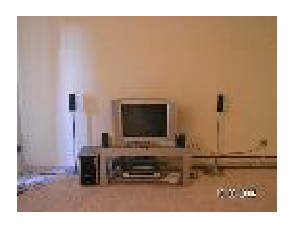
\includegraphics[width=0.19\columnwidth]{img/2007_002132}}{Raw}
  \subsubfloat{
\includegraphics[width=0.19\columnwidth]{img/2007_002132_label}}{Label}
  \subsubfloat{
\includegraphics[width=0.19\columnwidth]{img/2007_002132_up_pred}}{Complete}
  \subsubfloat{
\includegraphics[width=0.19\columnwidth]{img/2007_002132_exp_pred}}{ExpU.}
  \subsubfloat{
\includegraphics[width=0.19\columnwidth]{img/2007_002132_low_pred}}{CrossEnt.}
  \subsubfloat{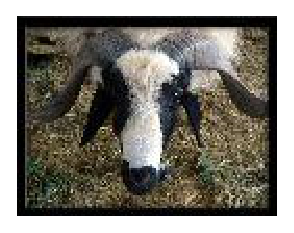
\includegraphics[width=0.19\columnwidth]{img/2007_002618}}{Raw}%
  \subsubfloat{
\includegraphics[width=0.19\columnwidth]{img/2007_002618_label}}{Label}
  \subsubfloat{
\includegraphics[width=0.19\columnwidth]{img/2007_002618_up_pred}}{Complete}
  \subsubfloat{
\includegraphics[width=0.19\columnwidth]{img/2007_002618_exp_pred}}{ExpU.}
  \subsubfloat{
\includegraphics[width=0.19\columnwidth]{img/2007_002618_low_pred}}{CrossEnt.}
  \end{minipage}
\caption{
Selective predictions made by models trained with the sigmoidal negative loss and the cross-entropy loss.
This figure presented two selective images for which the model trained with the cross entropy loss failed to segment objects, and the one with sigmoidal negative loss succeed.
}
\label{fig:pusegment}
\end{figure}


\section{Discussion}
\label{sec:discussion}

%%%%%%%%%%%%%%%%%%%%%%%%%%%%%%%%%%%%%%%%%%%%%%%%%%%%%%%%%%%%%%%%%%%%%%
%%%%%%%% Influence of label noises
%%%%%%%%%%%%%%%%%%%%%%%%%%%%%%%%%%%%%%%%%%%%%%%%%%%%%%%%%%%%%%%%%%%%%%

We assumed incomplete segmentation, misclassification and false segmentation of objects had occurred independently to the exact shape and appearance of the objects when we synthesized the segmentation noises stochastically in our experiments.
However, some categories can be more likely to be misclassified due to its ambiguity in shapes or appearances in practice, such as bear and teddy bear.
Similarly,  ambiguous objects can have a higher probability of being missing than easily recognizable objects.
A real dataset with both clean and noisy segmentation would be valuable to evaluate the influence of noises on feature transferability further.
% In addtion, we exluded segmenting errors such as imprecise boundaries, oversegmenting or undersegmenting the objects from study because they are a bit more complex to synthesize than the three classification errors.

%%%%%%%%%%%%%%%%%%%%%%%%%%%%%%%%%%%%%%%%%%%%%%%%%%%%%%%%%%%%%%%%%%%%%%
%%%%%%%% Binarizing classes
%%%%%%%%%%%%%%%%%%%%%%%%%%%%%%%%%%%%%%%%%%%%%%%%%%%%%%%%%%%%%%%%%%%%%%

We proposed to binarize or categorize classes to produce accurate but imprecise labels when misclassification of segments dominates a small pre-training dataset.
The result feature transferability depends on whether the inaccurate labels or the imprecise labels is more severe in the decrease of feature transferability.
In our experiment, the limited amounts of training images, the low-resolution of images and the constraint capacity of the FCN-AlexNet model may explain that more precise labels cannot improve the fine-tuning performance for the pre-trained models.
In general, a trade-off between precise but less ccurate labels and more accurate but less precise labels need to be made to train better transferable features, given a particular dataset.


%%%%%%%%%%%%%%%%%%%%%%%%%%%%%%%%%%%%%%%%%%%%%%%%%%%%%%%%%%%%%%%%%%%%%%
%%%%%%%% Sigmoidal loss
%%%%%%%%%%%%%%%%%%%%%%%%%%%%%%%%%%%%%%%%%%%%%%%%%%%%%%%%%%%%%%%%%%%%%%

We argued that not over-punishing confident, positive predictions for samples with negative labels can be beneficial by assuming the confident predictions are more likely to be mislabeled given a nonrandom model.
However, there can also be disadvantageous for over-excusing losses for confident predictions.
One typical problem is that a model made bad predictions with confidence will keep emphasizing its wrong predictions.
Therefore, the threshold between punishing and excusing a certain model for make confident contrary predictions need to be tuned appropriately to achieve both high precision and high recall.
Unfortunately, the sigmoidal negative loss has no such hyperparameter to tune, which can be a direction to improve it in the future.
For example, the Focal Loss\cite{lin2017focal} could be a parametrizable alternative of the sigmoidal negative loss.

Besides, applying the sigmoidal negative loss to segmentation assumes that the foreground-to-background mislabeling for each pixel occurred independently.
This assumption made it possible to implement sigmoidal negative loss directly to classification for individual pixels.
However, there is normally a spatial dependence for noises in pixel labels which may help improve the spatial consistency of predictions.
Therefore, future works may be possible to make use of the spatial dependence of pixel label noises.

% Upside:
% \begin{itemize}
%   \item treat easy/hard classifications differently
%   \item not over-punish confident positive prediction for negatively labeled examples
% \end{itemize}
%
% Downside:
% \begin{itemize}
%   \item Optimization diffilculty introduced as a result of non-convex objective
% \end{itemize}

% The sigmoidal loss was introduced in \cite{tax2016class} to get rid of the effect of outliers.
% In our case, the negative examples given confident predictions by classifier can be considered as outliers.

% Another challenge of difficulty encountered in implementingin extending sigmoidal negative loss to multi-class scenario

% \paragraph{The relationship between PU learning and Imbalanced learning}

% Imbalanced
% Easily classified negatives comprise
% the majority of the loss and dominate the gradient. While
% α balances the importance of positive/negative examples, it
% does not differentiate between easy/hard examples

% \paragraph{Future works}
%
% \begin{itemize}
%   \item Parameterizing exponential unlabeled loss to determine boundaries of confident and unconfident predictions
%   \item Take into account label noise spatial dependence for neighboring pixels
%   \item Experiment with over-segmentation and under-segmentation noises (negative influence expected)
%   \item Experiment with real datasets
% \end{itemize}


\section{Conclusion}
\label{sec:conclusion}

We studied how to pre-train transferable convolutional weights in the presence of inexhaustive segmentation, misclassification and false segmentation.
We discovered that including false segmentations of meaningful objects for pre-training had little impact on the fine-tuning performance of transferred weights
By contrast, misclassification noises can have negative impacts on feature transferability, but binarizing classes to foreground and background can produce accurate but not necessarily precise labels to train better transferable features.
We presented that for a small pre-training set, binarizing classes can recover the negative influence of misclassification of object segments on the fine-tuning performance of the transferred models.
Inexhaustive segmentation can also negatively affect feature transferability of the pre-trained model.
The decrease of the fine-tuning performance due to the unsegmented objects in the pre-training set can be compensated by modifying the loss function for deep learning models.
We then proposed a class-dependent loss to not over-punish the confident positive predictions for examples with negative labels.
The proposed sigmoidal negative loss was demonstrated to improve both the pre-training and fine-tuning performance of models pre-trained in the presence of inexhaustive segmentations.



{\small
\bibliographystyle{plain}
\bibliography{references}
}

\clearpage
\newpage
\appendix


%%%%%%%%%%%%%%%%%%%%%%%%%%%%%%%%%%%%%%%%%%%%%%%%%%%%%%%%%%%%%%%%%%%%%%
%%%%%%%%%%%%%%%% Convolutional Networks for Semantic Segmentation
%%%%%%%%%%%%%%%%%%%%%%%%%%%%%%%%%%%%%%%%%%%%%%%%%%%%%%%%%%%%%%%%%%%%%%

\section{Convolutional Networks for Semantic Segmentation}



%%%%%%%%%%%%%%%%%%%%%%%%%%%%%%%%%%%%%%%%%%%%%%%%%%%%%%%%%%%%%%%%%%%%%%
%%%%%%%%%%%%%%%% Deep Learning with label noise
%%%%%%%%%%%%%%%%%%%%%%%%%%%%%%%%%%%%%%%%%%%%%%%%%%%%%%%%%%%%%%%%%%%%%%

\section{Deep Learning with Label Noise}
NNAR, NAR, NCAR



%%%%%%%%%%%%%%%%%%%%%%%%%%%%%%%%%%%%%%%%%%%%%%%%%%%%%%%%%%%%%%%%%%%%%%
%%%%%%%%%%%%%%%%
%%%%%%%%%%%%%%%%%%%%%%%%%%%%%%%%%%%%%%%%%%%%%%%%%%%%%%%%%%%%%%%%%%%%%%

\section{Evaluation metrics}

(overall) accuracy
$$ \text{accuracy} = \frac{\text{true pos. + true neg.}}{\text{true pos. + false pos. + true neg. + false neg.}}$$

precision
$$\text{precision} = \frac{\text{true pos.}}{\text{true pos. + false pos.}}$$

recall
$$\text{recall} = \frac{\text{true pos.}}{\text{true pos. + false neg.}}$$

f1-score
$$F_1 = 2 \cdot \frac{\text{precision} \cdot \text{recall}}{\text{precision}+\text{recall}}$$

intersection over union (IU)
$$ \text{IU} = \frac{\text{true pos.}}{\text{true pos. + false pos. + false neg.}}$$

%%%%%%%%%%%%%%%%%%%%%%%%%%%%%%%%%%%%%%%%%%%%%%%%%%%%%%%%%%%%%%%%%%%%%%
%%%%%%%%%%%%%%%% Appendix Results                     %%%%%%%%%%%%%%%%
%%%%%%%%%%%%%%%%%%%%%%%%%%%%%%%%%%%%%%%%%%%%%%%%%%%%%%%%%%%%%%%%%%%%%%

\section{Additional Results}
%%%%%%%% FIGURE Number of training categories
\begin{figure}[t]
\centering
   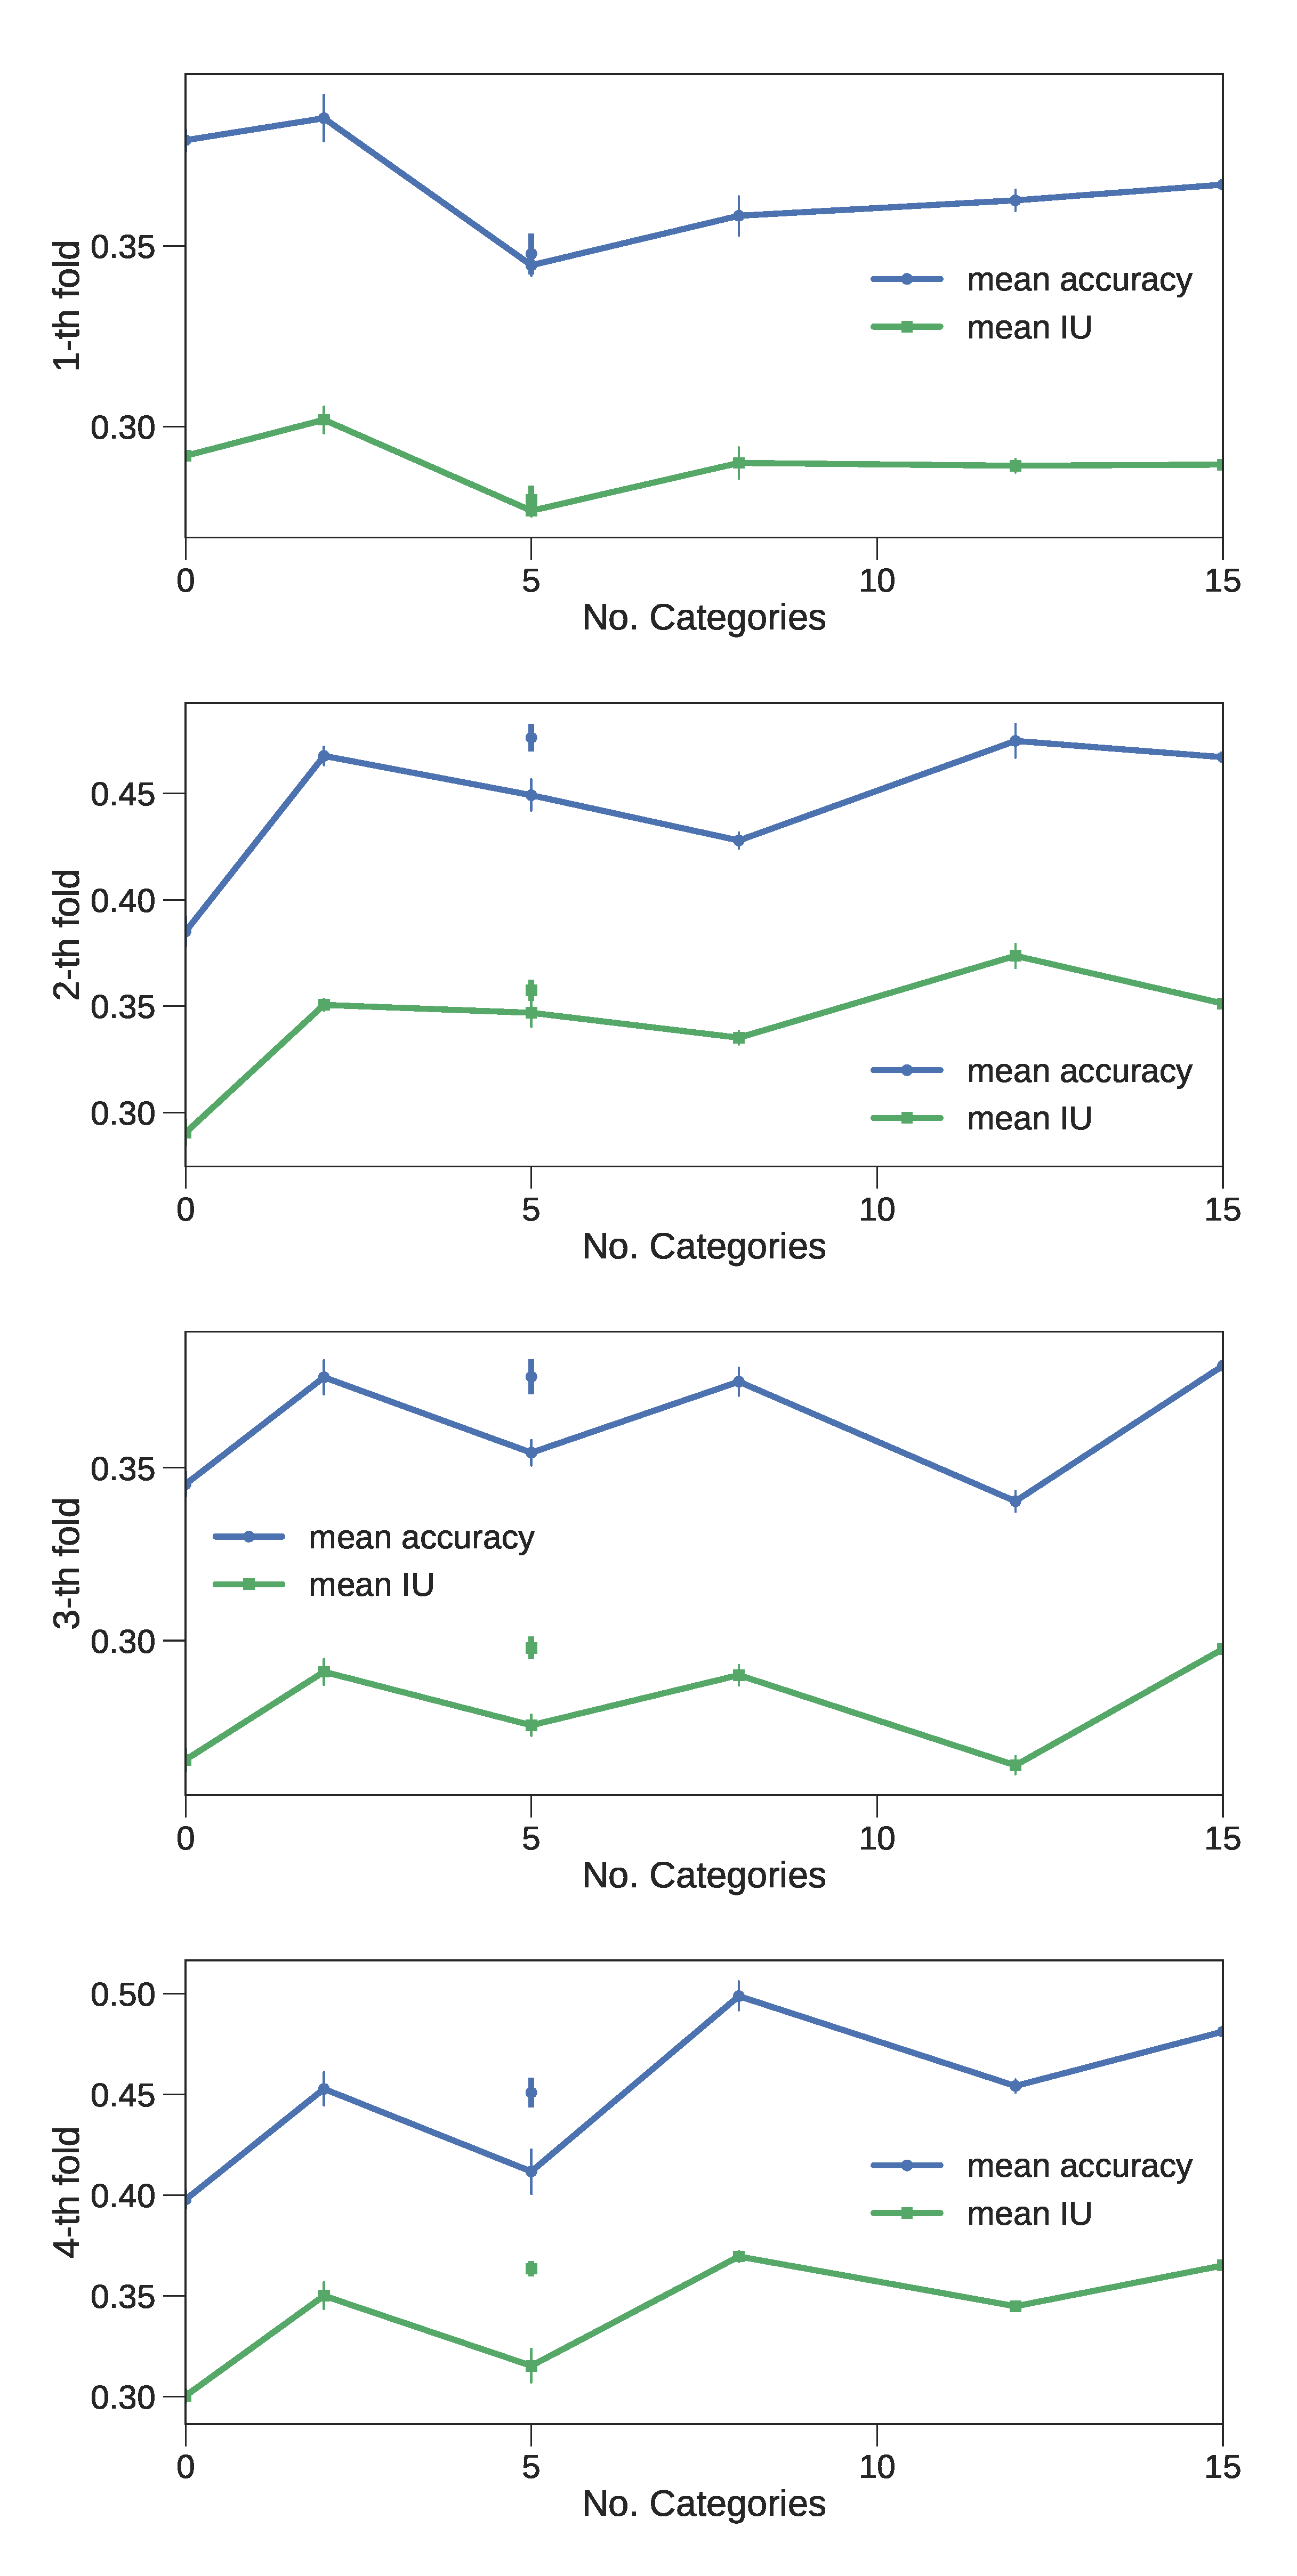
\includegraphics[width=\linewidth]{img/num_classes_folds.eps}
\caption{The influence of number of pre-training categories on performance of fine-tuned models for each fold, addition to Figure \ref{fig:categories}.}
\label{fig:classesfold}
\end{figure}


\end{document}
